% =====================================================================
%  Algorithmic Equity and Capital Allocation
%  Chicago lead service line replacement (LSLR)
%  Build:  xelatex main && bibtex main && xelatex main && xelatex main
%          (or: latexmk -xelatex main.tex)
%  Inputs generated by src/analysis.py: results.tex, tab_*.tex
% =====================================================================
\documentclass[11pt]{article}
\usepackage[margin=1in]{geometry}
\usepackage{amsmath,amsthm,mathtools}
\usepackage{fontspec}
\usepackage[math-style=TeX]{unicode-math}
\setmainfont{Times New Roman}
\setsansfont{Times New Roman}
\setmonofont{Times New Roman}
\setmathfont{TeX Gyre Termes Math}
\setmathfont[range={up/{latin,Latin,num,greek,Greek}}]{Times New Roman}
\setmathfont[range={it/{latin,Latin,greek,Greek}}]{Times New Roman Italic}
\setmathfont[range={bfup/{latin,Latin,num}}]{Times New Roman Bold}
\setmathfont[range={bfit/{latin,Latin}}]{Times New Roman Bold Italic}
\usepackage[authoryear,round]{natbib}
\usepackage{booktabs,tabularx,array,multirow,threeparttable}
\usepackage{graphicx}
\usepackage{xcolor}
\usepackage{listings}
\usepackage[ruled,vlined,linesnumbered]{algorithm2e}
\usepackage{siunitx}
\usepackage{enumitem}
\usepackage{caption}
\captionsetup{font=small,labelfont=bf,labelsep=period}
\usepackage[colorlinks=true,linkcolor=blue!45!black,citecolor=blue!45!black,urlcolor=blue!45!black]{hyperref}
\usepackage[nameinlink,capitalise]{cleveref}
\crefname{equation}{Eq.}{Eqs.}

\graphicspath{{../figures/}}
\sisetup{group-separator={,},group-minimum-digits=4}
\newtheorem{proposition}{Proposition}
\setlength{\parskip}{0.25em}
\definecolor{codebg}{HTML}{F7F7F7}
\lstset{basicstyle=\rmfamily\scriptsize,backgroundcolor=\color{codebg},frame=single,
  rulecolor=\color{black!20},breaklines=true,columns=fullflexible,keepspaces=true,
  keywordstyle=\bfseries,commentstyle=\itshape\color{black!60},showstringspaces=false,
  numbers=left,numberstyle=\tiny\color{black!40},xleftmargin=1.5em,upquote=true}

% auto-generated by src/analysis.py; do not edit
\newcommand{\SQHarm}{24.27}
\newcommand{\SQCost}{11.50}
\newcommand{\SQSocial}{35.77}
\newcommand{\SQNominal}{16.08}
\newcommand{\SQGap}{-0.68}
\newcommand{\SQWait}{12.4}
\newcommand{\SQWaitEJ}{12.1}
\newcommand{\SQWaitNonEJ}{12.5}
\newcommand{\SQGini}{0.062}
\newcommand{\SQAtkOne}{0.013}
\newcommand{\SQConc}{-0.015}
\newcommand{\SQDone}{0.901}
\newcommand{\SQExposure}{1.23}
\newcommand{\SQCompletion}{2048}
\newcommand{\SQGapAbs}{0.7}
\newcommand{\SQDonePct}{90.1}
\newcommand{\SQBlock}{0}
\newcommand{\PRHarm}{24.30}
\newcommand{\PRCost}{11.51}
\newcommand{\PRSocial}{35.80}
\newcommand{\PRNominal}{16.08}
\newcommand{\PRGap}{+0.00}
\newcommand{\PRWait}{12.4}
\newcommand{\PRWaitEJ}{12.4}
\newcommand{\PRWaitNonEJ}{12.4}
\newcommand{\PRGini}{0.000}
\newcommand{\PRAtkOne}{-0.000}
\newcommand{\PRConc}{+0.000}
\newcommand{\PRDone}{0.902}
\newcommand{\PRExposure}{1.23}
\newcommand{\PRCompletion}{2048}
\newcommand{\PRGapAbs}{0.0}
\newcommand{\PRDonePct}{90.2}
\newcommand{\PRBlock}{0}
\newcommand{\POHarm}{20.67}
\newcommand{\POCost}{11.50}
\newcommand{\POSocial}{32.18}
\newcommand{\PONominal}{16.08}
\newcommand{\POGap}{-4.22}
\newcommand{\POWait}{12.4}
\newcommand{\POWaitEJ}{9.0}
\newcommand{\POWaitNonEJ}{14.8}
\newcommand{\POGini}{0.361}
\newcommand{\POAtkOne}{0.337}
\newcommand{\POConc}{-0.212}
\newcommand{\PODone}{0.901}
\newcommand{\POExposure}{1.02}
\newcommand{\POCompletion}{2048}
\newcommand{\POGapAbs}{4.2}
\newcommand{\PODonePct}{90.1}
\newcommand{\POBlock}{0}
\newcommand{\CMHarm}{21.31}
\newcommand{\CMCost}{9.58}
\newcommand{\CMSocial}{30.88}
\newcommand{\CMNominal}{13.04}
\newcommand{\CMGap}{-1.69}
\newcommand{\CMWait}{11.4}
\newcommand{\CMWaitEJ}{10.0}
\newcommand{\CMWaitNonEJ}{12.4}
\newcommand{\CMGini}{0.318}
\newcommand{\CMAtkOne}{0.218}
\newcommand{\CMConc}{-0.076}
\newcommand{\CMDone}{1.000}
\newcommand{\CMExposure}{1.05}
\newcommand{\CMCompletion}{2046}
\newcommand{\CMGapAbs}{1.7}
\newcommand{\CMDonePct}{100.0}
\newcommand{\CMBlock}{100}
\newcommand{\HWHarm}{18.12}
\newcommand{\HWCost}{9.77}
\newcommand{\HWSocial}{27.89}
\newcommand{\HWNominal}{13.05}
\newcommand{\HWGap}{-3.58}
\newcommand{\HWWait}{10.7}
\newcommand{\HWWaitEJ}{7.8}
\newcommand{\HWWaitNonEJ}{12.8}
\newcommand{\HWGini}{0.365}
\newcommand{\HWAtkOne}{0.156}
\newcommand{\HWConc}{-0.211}
\newcommand{\HWDone}{1.000}
\newcommand{\HWExposure}{0.87}
\newcommand{\HWCompletion}{2046}
\newcommand{\HWGapAbs}{3.6}
\newcommand{\HWDonePct}{100.0}
\newcommand{\HWBlock}{100}
\newcommand{\EWHarm}{18.76}
\newcommand{\EWCost}{9.88}
\newcommand{\EWSocial}{28.64}
\newcommand{\EWNominal}{13.20}
\newcommand{\EWGap}{-3.60}
\newcommand{\EWWait}{10.7}
\newcommand{\EWWaitEJ}{7.4}
\newcommand{\EWWaitNonEJ}{13.2}
\newcommand{\EWGini}{0.314}
\newcommand{\EWAtkOne}{0.135}
\newcommand{\EWConc}{-0.245}
\newcommand{\EWDone}{1.000}
\newcommand{\EWExposure}{0.92}
\newcommand{\EWCompletion}{2046}
\newcommand{\EWGapAbs}{3.6}
\newcommand{\EWDonePct}{100.0}
\newcommand{\EWBlock}{99}
\newcommand{\ECHarm}{18.57}
\newcommand{\ECCost}{9.84}
\newcommand{\ECSocial}{28.41}
\newcommand{\ECNominal}{13.15}
\newcommand{\ECGap}{-3.92}
\newcommand{\ECWait}{10.7}
\newcommand{\ECWaitEJ}{7.2}
\newcommand{\ECWaitNonEJ}{13.2}
\newcommand{\ECGini}{0.345}
\newcommand{\ECAtkOne}{0.148}
\newcommand{\ECConc}{-0.263}
\newcommand{\ECDone}{1.000}
\newcommand{\ECExposure}{0.90}
\newcommand{\ECCompletion}{2046}
\newcommand{\ECGapAbs}{3.9}
\newcommand{\ECDonePct}{100.0}
\newcommand{\ECBlock}{100}
\newcommand{\DWHarm}{18.85}
\newcommand{\DWCost}{9.78}
\newcommand{\DWSocial}{28.63}
\newcommand{\DWNominal}{13.05}
\newcommand{\DWGap}{-6.53}
\newcommand{\DWWait}{10.7}
\newcommand{\DWWaitEJ}{5.9}
\newcommand{\DWWaitNonEJ}{14.2}
\newcommand{\DWGini}{0.359}
\newcommand{\DWAtkOne}{0.157}
\newcommand{\DWConc}{-0.330}
\newcommand{\DWDone}{1.000}
\newcommand{\DWExposure}{0.92}
\newcommand{\DWCompletion}{2046}
\newcommand{\DWGapAbs}{6.5}
\newcommand{\DWDonePct}{100.0}
\newcommand{\DWBlock}{100}
\newcommand{\HRtwoHarm}{18.12}
\newcommand{\HRtwoCost}{9.77}
\newcommand{\HRtwoSocial}{27.90}
\newcommand{\HRtwoNominal}{13.05}
\newcommand{\HRtwoGap}{-3.59}
\newcommand{\HRtwoWait}{10.7}
\newcommand{\HRtwoWaitEJ}{7.8}
\newcommand{\HRtwoWaitNonEJ}{12.8}
\newcommand{\HRtwoGini}{0.365}
\newcommand{\HRtwoAtkOne}{0.155}
\newcommand{\HRtwoConc}{-0.211}
\newcommand{\HRtwoDone}{1.000}
\newcommand{\HRtwoExposure}{0.87}
\newcommand{\HRtwoCompletion}{2045}
\newcommand{\HRtwoGapAbs}{3.6}
\newcommand{\HRtwoDonePct}{100.0}
\newcommand{\HRtwoBlock}{100}
\newcommand{\HRsevenHarm}{18.12}
\newcommand{\HRsevenCost}{9.77}
\newcommand{\HRsevenSocial}{27.89}
\newcommand{\HRsevenNominal}{13.04}
\newcommand{\HRsevenGap}{-3.61}
\newcommand{\HRsevenWait}{10.7}
\newcommand{\HRsevenWaitEJ}{7.8}
\newcommand{\HRsevenWaitNonEJ}{12.8}
\newcommand{\HRsevenGini}{0.366}
\newcommand{\HRsevenAtkOne}{0.159}
\newcommand{\HRsevenConc}{-0.212}
\newcommand{\HRsevenDone}{1.000}
\newcommand{\HRsevenExposure}{0.87}
\newcommand{\HRsevenCompletion}{2046}
\newcommand{\HRsevenGapAbs}{3.6}
\newcommand{\HRsevenDonePct}{100.0}
\newcommand{\HRsevenBlock}{100}
\newcommand{\HChHarm}{18.24}
\newcommand{\HChCost}{9.77}
\newcommand{\HChSocial}{28.01}
\newcommand{\HChNominal}{13.05}
\newcommand{\HChGap}{-3.74}
\newcommand{\HChWait}{10.7}
\newcommand{\HChWaitEJ}{7.8}
\newcommand{\HChWaitNonEJ}{12.8}
\newcommand{\HChGini}{0.367}
\newcommand{\HChAtkOne}{0.163}
\newcommand{\HChConc}{-0.209}
\newcommand{\HChDone}{1.000}
\newcommand{\HChExposure}{0.86}
\newcommand{\HChCompletion}{2046}
\newcommand{\HChGapAbs}{3.7}
\newcommand{\HChDonePct}{100.0}
\newcommand{\HChBlock}{100}
\newcommand{\HHiHarm}{18.16}
\newcommand{\HHiCost}{9.77}
\newcommand{\HHiSocial}{27.93}
\newcommand{\HHiNominal}{13.05}
\newcommand{\HHiGap}{-3.32}
\newcommand{\HHiWait}{10.7}
\newcommand{\HHiWaitEJ}{7.9}
\newcommand{\HHiWaitNonEJ}{12.7}
\newcommand{\HHiGini}{0.364}
\newcommand{\HHiAtkOne}{0.155}
\newcommand{\HHiConc}{-0.207}
\newcommand{\HHiDone}{1.000}
\newcommand{\HHiExposure}{0.88}
\newcommand{\HHiCompletion}{2045}
\newcommand{\HHiGapAbs}{3.3}
\newcommand{\HHiDonePct}{100.0}
\newcommand{\HHiBlock}{100}
\newcommand{\HHuHarm}{18.41}
\newcommand{\HHuCost}{9.77}
\newcommand{\HHuSocial}{28.18}
\newcommand{\HHuNominal}{13.05}
\newcommand{\HHuGap}{-2.49}
\newcommand{\HHuWait}{10.7}
\newcommand{\HHuWaitEJ}{8.1}
\newcommand{\HHuWaitNonEJ}{12.6}
\newcommand{\HHuGini}{0.353}
\newcommand{\HHuAtkOne}{0.157}
\newcommand{\HHuConc}{-0.171}
\newcommand{\HHuDone}{1.000}
\newcommand{\HHuExposure}{0.90}
\newcommand{\HHuCompletion}{2046}
\newcommand{\HHuGapAbs}{2.5}
\newcommand{\HHuDonePct}{100.0}
\newcommand{\HHuBlock}{100}
\newcommand{\DecTotal}{7.88}
\newcommand{\DecOrdering}{3.59}
\newcommand{\DecClustering}{4.29}
\newcommand{\DecHarmTotal}{6.15}
\newcommand{\DecCostTotal}{1.73}
\newcommand{\DecCmVsSq}{4.89}
\newcommand{\SQAltCost}{9.14}
\newcommand{\SQAltSocial}{33.41}
\newcommand{\SavingAlt}{5.52}
\newcommand{\SavingAltPct}{17}
\newcommand{\RefCostShareGain}{61}
\newcommand{\DecOrderPct}{46}
\newcommand{\DecClusterPct}{54}
\newcommand{\GainPct}{22.0}
\newcommand{\MaxGapMusd}{223}
\newcommand{\MedGapMusd}{32}
\newcommand{\FrontMinGap}{-7.58}
\newcommand{\FrontMinGapCost}{0.51}
\newcommand{\DomZeroCost}{0.22}
\newcommand{\PsaN}{2,000}
\newcommand{\PsaHWbeatsSQ}{100.0}
\newcommand{\PsaHWbest}{100.0}
\newcommand{\PsaSaveMed}{9.28}
\newcommand{\PsaSaveLo}{4.43}
\newcommand{\PsaSaveHi}{17.28}
\newcommand{\PsaBcrMed}{4.85}
\newcommand{\PsaBcrLo}{2.02}
\newcommand{\PsaBcrHi}{10.44}
\newcommand{\PsaBcrBelowOne}{0.1}
\newcommand{\ConsN}{608}
\newcommand{\ConsAttempts}{13,330}
\newcommand{\ConsRefusals}{2,974}
\newcommand{\ConsIRR}{1.057}
\newcommand{\ConsIRRp}{0.040}
\newcommand{\ConsIRRlo}{1.003}
\newcommand{\ConsIRRhi}{1.115}
\newcommand{\PRefOwner}{20.2}
\newcommand{\PRefRenter}{25.0}
\newcommand{\RefCost}{4.84}
\newcommand{\RefCostEJ}{66}
\newcommand{\RefRho}{21.9}
\newcommand{\RefRhoQF}{23.5}
\newcommand{\RefRhoQO}{20.6}
\newcommand{\RhoSviLate}{0.61}
\newcommand{\RhoSviLateCI}{[0.43, 0.75]}
\newcommand{\RhoSviLong}{0.64}
\newcommand{\RhoSviLongCI}{[0.46, 0.77]}
\newcommand{\RhoHolcDLate}{0.21}
\newcommand{\RhoHolcDLateCI}{[-0.03, 0.44]}
\newcommand{\RhoHolcDLong}{0.41}
\newcommand{\RhoHolcDLongCI}{[0.19, 0.60]}
\newcommand{\RhoKidsLate}{0.17}
\newcommand{\RhoKidsLateCI}{[-0.04, 0.40]}
\newcommand{\RhoKidsLong}{0.04}
\newcommand{\RhoKidsLongCI}{[-0.17, 0.25]}
\newcommand{\RhoActionLate}{0.28}
\newcommand{\RhoActionLateCI}{[0.07, 0.48]}
\newcommand{\RhoActionLong}{0.00}
\newcommand{\RhoActionLongCI}{[-0.20, 0.20]}
\newcommand{\ImpAUC}{0.903}
\newcommand{\ImpN}{158,389}
\newcommand{\ImpBase}{82.8}
\newcommand{\ImpBrier}{0.081}
\newcommand{\ImpBrierNull}{0.143}
\newcommand{\NCa}{76}
\newcommand{\NLines}{491,406}
\newcommand{\NAction}{412,433}
\newcommand{\NL}{150,860}
\newcommand{\NGRR}{10,525}
\newcommand{\NU}{251,048}
\newcommand{\NNL}{78,973}
\newcommand{\NLeadExp}{371,181}
\newcommand{\PULead}{83.6}
\newcommand{\NReplaced}{10,638}
\newcommand{\NRefused}{3,026}
\newcommand{\NHighRisk}{2,676}
\newcommand{\NTracts}{800}
\newcommand{\NZones}{160}
\newcommand{\KidsServed}{103,616}
\newcommand{\AdultsServed}{1,124,587}
\newcommand{\KidsCity}{180,915}
\newcommand{\HQA}{4,716}
\newcommand{\ReplQA}{23.4}
\newcommand{\RefQA}{5.8}
\newcommand{\KidsQA}{0.22}
\newcommand{\RentQA}{34}
\newcommand{\HQB}{5,334}
\newcommand{\ReplQB}{27.0}
\newcommand{\RefQB}{6.9}
\newcommand{\KidsQB}{0.20}
\newcommand{\RentQB}{38}
\newcommand{\HQC}{5,823}
\newcommand{\ReplQC}{23.0}
\newcommand{\RefQC}{5.6}
\newcommand{\KidsQC}{0.23}
\newcommand{\RentQC}{36}
\newcommand{\HQD}{7,102}
\newcommand{\ReplQD}{25.6}
\newcommand{\RefQD}{8.6}
\newcommand{\KidsQD}{0.28}
\newcommand{\RentQD}{52}
\newcommand{\HQE}{7,668}
\newcommand{\ReplQE}{30.2}
\newcommand{\RefQE}{9.8}
\newcommand{\KidsQE}{0.33}
\newcommand{\RentQE}{57}
\newcommand{\HMeanChild}{3,189}
\newcommand{\HMeanCentral}{6,119}
\newcommand{\HMeanHigh}{10,820}
\newcommand{\VChild}{14,116}
\newcommand{\VAdult}{1,204}
\newcommand{\VAdultHigh}{3,135}
\newcommand{\BCRChildEpaTwo}{15.19}
\newcommand{\BCRChildEpaThree}{13.30}
\newcommand{\BCRChildEpaSeven}{8.42}
\newcommand{\BCRChildTenTwo}{7.14}
\newcommand{\BCRChildTenThree}{6.25}
\newcommand{\BCRChildTenSeven}{3.96}
\newcommand{\BCRChildThirtyOneTwo}{2.30}
\newcommand{\BCRChildThirtyOneThree}{2.02}
\newcommand{\BCRChildThirtyOneSeven}{1.28}
\newcommand{\BCRChildThirtyNineTwo}{1.83}
\newcommand{\BCRChildThirtyNineThree}{1.60}
\newcommand{\BCRChildThirtyNineSeven}{1.01}
\newcommand{\BCRCentralEpaTwo}{29.16}
\newcommand{\BCRCentralEpaThree}{25.52}
\newcommand{\BCRCentralEpaSeven}{16.15}
\newcommand{\BCRCentralTenTwo}{13.70}
\newcommand{\BCRCentralTenThree}{11.99}
\newcommand{\BCRCentralTenSeven}{7.59}
\newcommand{\BCRCentralThirtyOneTwo}{4.42}
\newcommand{\BCRCentralThirtyOneThree}{3.87}
\newcommand{\BCRCentralThirtyOneSeven}{2.45}
\newcommand{\BCRCentralThirtyNineTwo}{3.51}
\newcommand{\BCRCentralThirtyNineThree}{3.08}
\newcommand{\BCRCentralThirtyNineSeven}{1.95}
\newcommand{\BCRHighEpaTwo}{51.56}
\newcommand{\BCRHighEpaThree}{45.12}
\newcommand{\BCRHighEpaSeven}{28.57}
\newcommand{\BCRHighTenTwo}{24.23}
\newcommand{\BCRHighTenThree}{21.21}
\newcommand{\BCRHighTenSeven}{13.43}
\newcommand{\BCRHighThirtyOneTwo}{7.82}
\newcommand{\BCRHighThirtyOneThree}{6.84}
\newcommand{\BCRHighThirtyOneSeven}{4.33}
\newcommand{\BCRHighThirtyNineTwo}{6.21}
\newcommand{\BCRHighThirtyNineThree}{5.44}
\newcommand{\BCRHighThirtyNineSeven}{3.44}
\newcommand{\TotalBudget}{14.5}
\newcommand{\EJShare}{42.2}


\newcommand{\Zs}{\mathcal{Z}}
\newcommand{\Ts}{\mathcal{T}}
\newcommand{\EJ}{\mathcal{E}}
\newcommand{\Qf}{\mathcal{Q}_5}
\newcommand{\BLL}{\mathrm{BLL}}
\newcommand{\SVI}{\mathrm{SVI}}
\newcommand{\ugdl}{\si{\micro\gram\per\deci\liter}}

\title{\textbf{Algorithmic Equity and Capital Allocation:}\\[2pt]
A Computational Optimization Framework for Chicago's $\sim$400,000 Lead Service Line
Replacements Across Economics, Environmental Justice, and Municipal Policy}
\author{Vikram Menon\\[2pt]\small Monta Vista High School, Cupertino, California, USA}
\date{\small Manuscript prepared for \emph{Environmental Science \& Policy}\quad|\quad October 2026}

\begin{document}
\maketitle

\begin{abstract}
\noindent\textbf{Context.} Chicago holds the largest lead service line (LSL) inventory of any
U.S. city. Its 2025 inventory lists \NLines{} service lines, of which \NAction{} are lead,
galvanized requiring replacement, or of unknown and suspected-lead material. This legacy of a
municipal code that required lead pipe until 1986 must now be retired within an approximately
twenty-year deferred schedule under the 2024 Lead and Copper Rule Improvements (LCRI), at a
reported \$31,000 to \$39,000 per line.
\textbf{Problem.} Under binding budgets and crew capacity, the sequence of replacement determines
who bears decades of residual exposure, what the program costs, and whether the deadline is met.
\textbf{Methods.} We join the address-level inventory to ACS, CDC/ATSDR Social Vulnerability
Index, HOLC redlining and Chicago Department of Public Health (CDPH) blood-lead data. We impute
unknown materials with a spatially cross-validated classifier (AUC \ImpAUC), and schedule
replacements across \NZones{} corridors and 20 years with a multi-objective mixed-integer linear
program. The objective prices health harm with the U.S. EPA's LCRI benefit methodology, captures
block-level economies of scale through a fixed-charge mobilization cost, and penalizes
vulnerability-weighted waiting; constraints encode capital budgets, crews, the LCRI pace and an
environmental-justice (EJ) non-discrimination floor. We trace the welfare--equity frontier, test
five equity frameworks, estimate the determinants of refusals of access, and propagate parameter
uncertainty through \PsaN{} Monte Carlo draws.
\textbf{Findings.} Continuing the 2021--2025 replacement pattern finishes in \SQCompletion{} and
carries a present-value social cost of \$\SQSocial{} billion. The welfare-optimal schedule finishes
on time and costs \$\HWSocial{} billion, a saving of \$\DecTotal{} billion (\GainPct\%), of which
\DecOrderPct\% comes from ordering by risk and \DecClusterPct\% from clustering work into block
programs. Because harm and vulnerability are correlated, the optimum serves the most vulnerable
quintile \HWGapAbs{} years earlier than the citywide mean; schedules that delay the vulnerable are
Pareto-dominated. Symmetric inequality indices rank these schedules backwards. Refusals of access
rise with renter share and cost an estimated \$\RefCost{} billion in delayed benefits, most of it
in EJ zones. Replacement passes a benefit--cost test in every benefit tier and discount rate
examined (BCR \BCRChildThirtyOneSeven{} to \BCRHighThirtyOneTwo{} at \$31,000).
\textbf{Policy.} We propose four ordinances: mandatory replacement with right of entry; zero-cost
replacement with an affordability rider; algorithmic transparency with a directional equity audit;
and unit-cost benchmarking with local hiring.
\par\medskip\noindent\textbf{Keywords:} lead service lines; environmental justice; mixed-integer
linear programming; cost--benefit analysis; social discount rate; split incentives;
infrastructure equity; Chicago
\end{abstract}

\paragraph{Highlights}
\begin{itemize}[nosep,leftmargin=1.2em]
\item Address-level 2025 inventory: \NAction{} Chicago service lines require action.
\item Risk ordering plus block clustering saves \$\DecTotal{} billion and meets the deadline.
\item The welfare optimum serves the most vulnerable first; delaying them is dominated.
\item Gini and Atkinson indices penalize progressive triage; use directional metrics.
\item Refusals of access, not sequencing, are the binding equity constraint.
\end{itemize}

\medskip\noindent\fbox{\parbox{\dimexpr\linewidth-2\fboxsep-2\fboxrule\relax}{\small
\textbf{Data and modeling statement.} Service-line counts, materials, locations, completed
replacements, refusals of access, demographics, vulnerability, redlining grades and historical
blood-lead screening are observed public data (\cref{sec:data}). Dose increments, unit costs,
mobilization cost, budgets and crew limits are modeling assumptions anchored to reported values
and are varied jointly in \cref{sec:psa}. Tap-water sampling is not public at address level, so
exposure is assumed uniform per lead line in the central case; a published tap-lead gradient is
tested as a sensitivity.}}

% =====================================================================
\section{Introduction}\label{sec:intro}
% =====================================================================
\subsection{Scale of the problem}
Chicago's lead problem is an institutional artifact before it is an engineering one. The city's
plumbing code required lead service lines, the pipe that connects a building to the water main,
for most residential construction until the 1986 Safe Drinking Water Act amendments banned lead
pipe nationally \citep{troesken2006}. The result is the largest LSL inventory of any U.S.
municipality. The inventory the Chicago Department of Water Management (CDWM) submitted to the
Illinois EPA in April 2025 lists 491,705 service lines: 150,864 lead, 10,526 galvanized requiring
replacement (GRR), 251,247 of unknown and suspected-lead material, and only 79,068 not lead
\citep{icn2025data}. Nationally, LSLs are concentrated in older Midwestern and Northeastern systems
\citep{cornwell2016}.

Progress has been slow relative to the stock. The inventory records \NReplaced{} completed
replacements dated 2021--2025, rising to about 4,750 in 2024, and the city planned roughly 10,000
replacements for 2026 \citep{wttw2025}. Reported unit costs average about \$31,000 per line:
roughly \$34,000 for block-level work and \$39,000 for one-off jobs, against an EPA national
estimate of \$4,700 and a peer-city range of \$6,000 to \$25,000 \citep{icn2026cost}. At these
prices the full program is a \$12 to \$14 billion capital commitment. The gap between block and
one-off costs is the first economic fact this paper builds on: the order of replacement changes
not only who is exposed but also what the program costs.

\subsection{Regulatory landscape}
Three instruments define the feasible set. First, the LCRI, finalized in October 2024, requires
systems to replace all lead and GRR lines within ten years of the November 1, 2027 compliance
date, lowers the lead action level to \SI{10}{\micro\gram\per\liter}, and permits deferred
deadlines where the required pace would exceed 39 replacements per 1,000 connections per year
\citep{epa2024lcri}. Chicago qualifies for a schedule of roughly twenty years \citep{cob2024}. EPA
estimated national benefits of \$13.49 to \$25.14 billion per year against costs of \$1.47 to
\$1.95 billion (2022 dollars, 2\% discount rate), with adult cardiovascular mortality and child IQ
the two largest benefit categories \citep{epa2024lcri,epa2024ea}. The rule is under challenge in
the D.C.\ Circuit, where oral argument was heard on September 30, 2026, and EPA has defended it
\citep{nrdc2026}. Second, the Illinois Lead Service Line Replacement and Notification Act (LSLRNA)
requires inventories, notification and replacement plans, with a 2077 deadline for systems above
99,999 lines \citep{ilga2021lslrna,wttw2024}, so the federal schedule binds. Third, the
Infrastructure Investment and Jobs Act appropriated \$15 billion nationally for LSLR through the
Drinking Water State Revolving Fund (DWSRF), of which about \$1.2 billion flowed to Illinois, and
dedicated funding ends in 2026 \citep{icn2026cost}. Chicago borrowed \$325 million through a
federal low-interest loan in 2023, of which no more than \$90 million had been spent by September
2025 \citep{wttw2025}. The binding constraints are therefore capital, crews and consent, not
legal authority.

\subsection{Environmental justice intersection}
Exposure is not spatially random. Chicago's South and West Sides combine historically redlined
neighborhoods, decades of disinvestment, older housing and majority Black and Hispanic
populations. HOLC grades had persistent effects on homeownership, housing values and segregation
\citep{aaronson2021}, and childhood lead poisoning in Chicago followed the same racial ecology for
two decades \citep{sampson2016}. Using 38,385 household tap samples, \citet{huynh2024} estimate
that 68\% of Chicago children under six live in homes with detectable tap lead, that a ten-point
increase in a block's Hispanic share is associated with an 11.2\% higher chance of contamination, and
that Black and Hispanic blocks were less likely to be tested. The CDC blood lead reference value
of 3.5~\ugdl{} \citep{ruckart2021} is a statistical marker, not a safe threshold: dose--response
is steepest at the lowest exposures \citep{lanphear2005,bellinger2008}, and even low BLLs reduce
later test scores \citep{aizer2018}. Flint showed how quickly water-borne lead appears in
children's blood when corrosion control fails \citep{hannaattisha2016}.

\subsection{The triage dilemma and contributions}
If every line will eventually be replaced, the policy question is sequencing under scarcity, a
scheduling problem with distributional stakes. Welfare economics prices the harm of delay,
operations research exploits the cost structure of clustered work, and environmental justice asks
whose exposure is prolonged. Treated separately they give conflicting advice. This paper unifies
them and makes four contributions.
\begin{enumerate}[nosep]
\item An empirical data architecture that joins the address-level inventory to census,
vulnerability, redlining and surveillance layers, with a validated model for unknown materials
(\cref{sec:data}).
\item A MOMILP whose objective terms are denominated in dollars using EPA's LCRI methodology and
whose constraints mirror Chicago's financial, operational and regulatory limits (\cref{sec:model}).
\item Evidence that, in Chicago, efficiency and vertical equity are complements over the relevant
range, that symmetric inequality indices misread progressive triage, and that the program is
robust to parameter uncertainty (\cref{sec:results,sec:econ}).
\item An estimate of the refusal-of-access problem and its welfare cost, and implementable
municipal policy (\cref{sec:econ,sec:policy}).
\end{enumerate}

% =====================================================================
\section{Data and ETL architecture}\label{sec:data}
% =====================================================================
\Cref{tab:dict} lists the input layers. All are public; \texttt{src/fetch\_data.py} downloads each
from its source, pinned to a repository commit where versioned, and records SHA-256 checksums.

\begin{table}[t]\centering\footnotesize
\caption{Data dictionary. All layers are harmonized to 2020 census tracts and then aggregated to
replacement zones.}\label{tab:dict}
\begin{tabularx}{\linewidth}{@{}>{\raggedright}p{2.7cm}>{\raggedright}p{3.1cm}p{1.3cm}>{\raggedright\arraybackslash}X@{}}
\toprule
Source & Dataset & Unit & Fields used and role in the model\\
\midrule
CDWM via Inside Climate News, Grist, WBEZ & 2025 service line inventory (491,705 records), geocoded & Address & material class, high-risk flag, identification source, replacement date, refusal of access; $N_z$, imputation, status quo, consent\\
CDC/ATSDR & Social Vulnerability Index 2022 & Tract & overall percentile \texttt{RPL\_THEMES}; $\SVI_z$, EJ zones, quintiles\\
U.S. Census Bureau & ACS 2019--2023 tables B01003, B09001, B25003, B25024, B25034 & Tract & population, children $<6$, tenure, units in structure, year built; $k_z$, $a_z$, renter share\\
Univ.\ of Richmond DSL & Mapping Inequality HOLC--2020 tract crosswalk & Tract & area share by HOLC grade; redlining legacy\\
CDPH (City Data Portal) & Child blood-lead screening, 1999--2013 & Community area & children screened and elevated; external validation\\
Inside Climate News & Tract and community-area boundaries & Polygon & spatial frame, maps\\
\bottomrule
\end{tabularx}
\end{table}

\paragraph{Inventory and geocoding.} The CDWM spreadsheet is joined record-by-record to the
geocoded file published by \citet{icn2025data}; the join reproduces the overall material
classification for 100\% of records. Restricting to tracts inside the city footprint leaves
\NLines{} lines: \NL{} lead, \NGRR{} GRR, \NU{} unknown and \NNL{} not lead. Under the LCRI,
unknown lines must be identified and, if lead, replaced, so all \NAction{} L, GRR and U lines enter
the scheduling problem.

\paragraph{Unknown-material imputation.} For each unknown line we estimate the probability that it
is lead using a gradient-boosted classifier trained on the \ImpN{} lines whose material was
verified in the field and that were never replaced (base rate \ImpBase\% lead). Features are
projected coordinates, the lead share among the 30 nearest verified neighbors (leave-one-out for
training rows), tract pre-1940 and pre-1986 housing shares, the share of units in one- to
four-unit structures, median income, race and ethnicity, and the high-risk flag. Five-fold
cross-validation with folds defined by tract prevents spatial leakage. Out-of-fold AUC is
\ImpAUC{} and the Brier score \ImpBrier{} against \ImpBrierNull{} for the base rate; calibration by
decile is close to the diagonal (\cref{fig:validation}c). The mean predicted probability for unknown
lines is \PULead\%, so the inventory implies about \NLeadExp{} lead lines among those requiring
action. Field-verified lines are not a random sample, and we treat this as a limitation.

\paragraph{Occupancy.} Small-diameter services that are typically lead serve one- to four-unit
buildings, so occupants per line are estimated as tract children under six (or adults) multiplied by
the share of housing units in such structures and divided by the tract's inventory count. This
places about \KidsServed{} of the city's \KidsCity{} children under six in buildings with lines
requiring action, consistent in magnitude with the 68\% exposure estimate of \citet{huynh2024}.

\paragraph{Replacement zones.} Water-main GIS is not public, so zones are formed by $k$-means on the
projected coordinates of the \NAction{} action lines ($k=\NZones$; about 2,600 lines and nine tracts
each). Each zone approximates a compact excavation corridor in which one crew mobilization can serve
many contiguous lines. Zone attributes are line-weighted means of tract attributes, and completed
replacements and refusals are attributed to the zone of the nearest action line.

\paragraph{What the data show.} \Cref{fig:maps} maps the layers. Lines requiring action make up
more than 85\% of service lines across most of the Northwest, Southwest and South Sides, and child
density per line is highest in the most vulnerable areas (\KidsQE{} children under six per line in
the most vulnerable quintile versus \KidsQA{} in the least). Two validation results anchor the
vulnerability measure. Across the \NCa{} community areas with screening data, line-weighted SVI is
strongly rank-correlated with the share of screened children found with elevated blood lead in
2009--2013 ($\rho=\RhoSviLate$, 95\% bootstrap CI \RhoSviLateCI), and the share of a community area
graded D by HOLC predicts its 1999--2013 blood-lead burden ($\rho=\RhoHolcDLong$,
\RhoHolcDLongCI). Redlining does not, however, predict more lead pipe today. Tracts dominated by D
grades have a lower share of lines requiring action than C-graded tracts (\cref{tab:holc}), plausibly
because urban renewal and later redevelopment replaced much of their pre-1986 housing. The
redlining legacy appears in health burden and vulnerability rather than in pipe material, an
important nuance for any EJ framing.

\begin{figure}[p]\centering
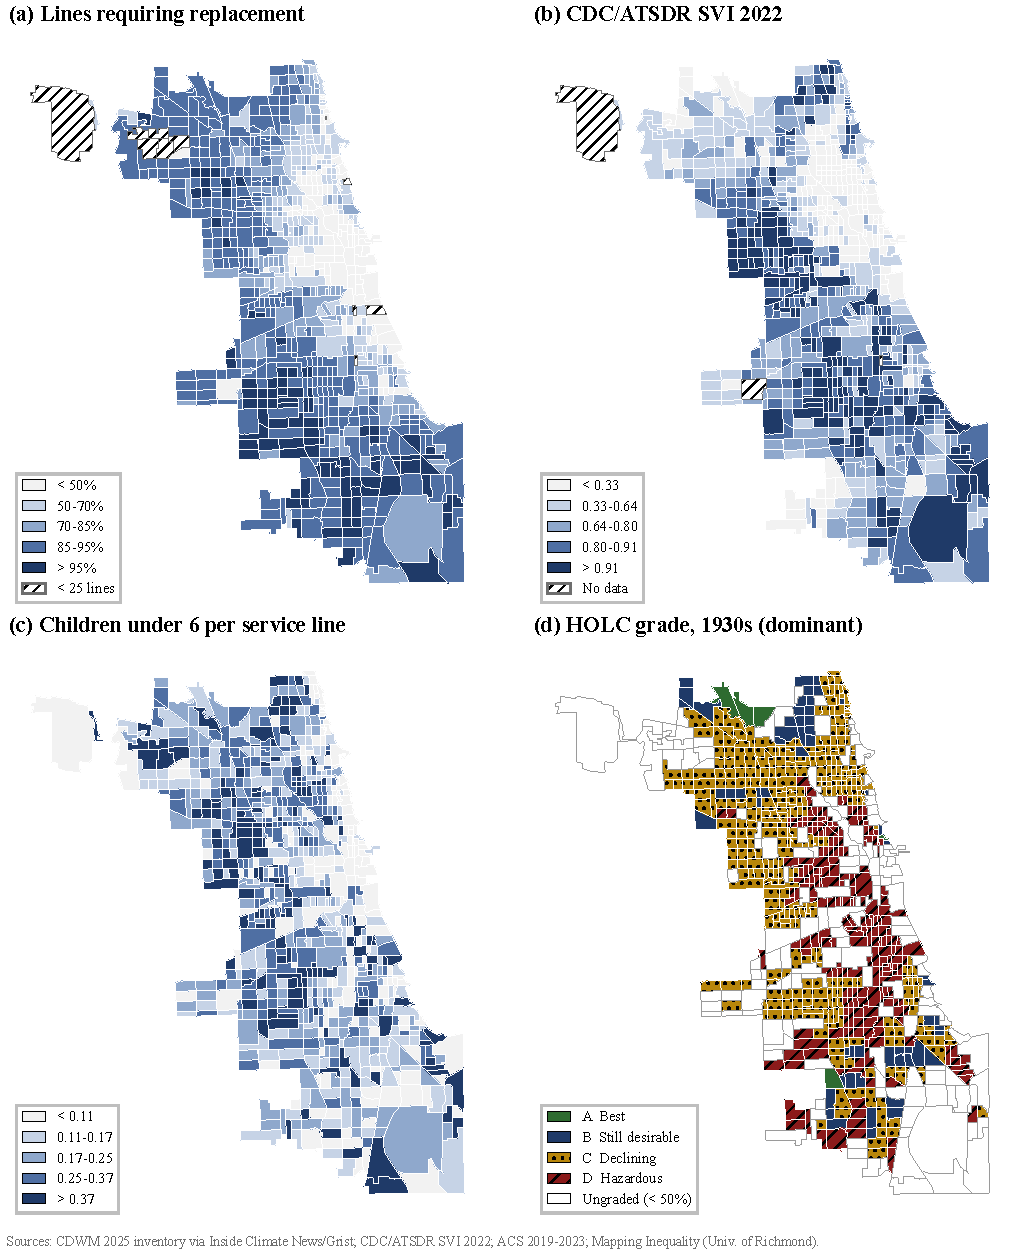
\includegraphics[width=0.93\linewidth]{fig01_inventory_maps.pdf}
\caption{Chicago's lead service line geography by 2020 census tract. Inventory shares were computed from the 2025 CDWM service line inventory geocoded to tracts (Section 2); vulnerability is the CDC/ATSDR SVI 2022 state percentile; child density combines ACS 2019--2023 tables B09001 and B25024 with inventory counts; HOLC grades come from the Mapping Inequality tract crosswalk. Lines requiring action exceed 85\% of service lines across most of the Northwest, Southwest and South Sides, and child density per line is highest where vulnerability is highest, while redlined (D) areas are not the areas with the most lead pipe today.}\label{fig:maps}
\end{figure}

\begin{table}[t]\centering\small
\caption{Inventory composition by dominant HOLC grade of the tract.}\label{tab:holc}
\begin{tabular}{@{}lrrrr@{}}
\toprule
Dominant grade & Tracts & Service lines & Requiring action & Mean SVI\\
\midrule
\csname @@input\endcsname tab_holc.tex 
\bottomrule
\end{tabular}
\end{table}

\begin{figure}[t]\centering
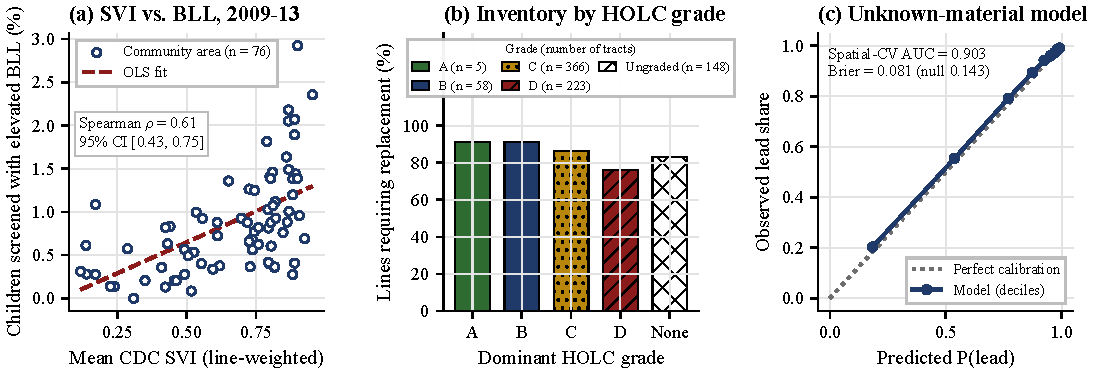
\includegraphics[width=\linewidth]{fig02_validation.pdf}
\caption{External and internal validation. (a) Line-weighted SVI against the share of screened children with elevated blood lead in 2009--2013 for 76 community areas (CDPH), with an OLS fit and a bootstrapped Spearman correlation (2,000 resamples). (b) Share of lines requiring action by dominant HOLC grade. (c) Reliability diagram of the unknown-material classifier from tract-blocked five-fold cross-validation on 158,389 field-verified lines. Vulnerability strongly predicts historical blood-lead burden ($\rho=0.61$), D-graded tracts hold proportionally fewer lead lines, and the imputation model is accurate (AUC 0.903) and well calibrated.}\label{fig:validation}
\end{figure}

% =====================================================================
\section{Mathematical model and computational formulation}\label{sec:model}
% =====================================================================
\subsection{Notation}
\begin{table}[h]\centering\small
\caption{Notation.}\label{tab:notation}
\begin{tabularx}{\linewidth}{@{}lX@{}}
\toprule
\multicolumn{2}{@{}l}{\emph{Sets}}\\
$z\in\Zs$ & replacement zones, $|\Zs|=\NZones$\\
$t\in\Ts=\{1,\dots,\bar T\}$ & years 2027--2046, $\bar T=20$\\
$\EJ\subset\Zs$ & environmental-justice zones, $\SVI_z$ at or above the 60th percentile (\EJShare\% of lines)\\
$\Qf\subset\Zs$ & most vulnerable quintile of lines\\
\multicolumn{2}{@{}l}{\emph{Parameters}}\\
$N_z$ & lines requiring action; $\pi^{\mathrm{L}}_z$ expected lead share (\cref{sec:data})\\
$k_z,\ a_z$ & children under six and adults per line\\
$h_z$ & monetized harm per unreplaced line-year (\$), \cref{eq:harm}\\
$c^B,\ c^O,\ F$ & block marginal cost, one-off cost, zone-year mobilization cost\\
$m_z$ & minimum block batch, $\min(250,N_z)$\\
$K_t,\ Y,\ B_t$ & annual line capacity, concurrent block crews, capital budget\\
$\pi_t,\ \delta_t$ & LCRI cumulative pace floor; mid-year discount factor $(1+r)^{-(t-1/2)}$\\
$\lambda,\ \omega_z$ & equity price; equity weight ($\SVI_z$ or convex variant)\\
\multicolumn{2}{@{}l}{\emph{Decision variables}}\\
$x_{z,t}\in[0,1]$ & share of zone $z$'s lines replaced in year $t$\\
$b_{z,t},\ o_{z,t}\geq0$ & lines replaced through block programs and one-off\\
$y_{z,t}\in\{0,1\}$ & block crew mobilized in zone $z$ in year $t$\\
$d_z\geq0$ & excess wait of zone $z$ above the citywide mean\\
\bottomrule
\end{tabularx}
\end{table}
Two derived quantities recur: the share of zone $z$ completed before year $t$ and the expected
completion year of its lines,
\begin{equation}
S_{z,t}=\sum_{s<t}x_{z,s},\qquad W_z=\sum_{t\in\Ts}t\,x_{z,t},\qquad
\bar W=\frac{1}{N}\sum_{z}N_zW_z,\quad N=\sum_z N_z .\label{eq:wait}
\end{equation}

\subsection{Damage functions}\label{sec:damage}
We follow the benefit methodology of EPA's LCRI economic analysis \citep{epa2024ea}.

\paragraph{Children.} IQ declines log-linearly in blood lead with the corrected pooled coefficient
$\beta=3.25$ \citep{lanphear2005,lanphear2019}; the original coefficient 2.70 is a sensitivity bound,
and \citet{crump2013} discuss the reanalysis. An LSL that raises a child's BLL from $B_0$ to
$B_0+\Delta B$ costs
\begin{equation}
\Delta IQ(B_0,\Delta B)=\beta\ln\!\Bigl(\frac{B_0+\Delta B}{B_0}\Bigr).\label{eq:iq}
\end{equation}
The logarithm is why low-level exposure matters: the marginal loss $\beta/\BLL$ is largest where
most children are (\cref{fig:damage}a). With $B_0=1.0$ and $\Delta B=0.8$~\ugdl{} over a six-year
early-childhood window, each child-year of exposure costs $\Delta IQ/6$ points, valued at EPA's
\$42,226 per IQ point (2022 dollars) and increased by 5\% for ADHD and special-education costs,
which is about EPA's ratio of ADHD to IQ benefits. This yields \$\VChild{} per exposed child-year.

\paragraph{Adults.} EPA's health impact function for cardiovascular (CVD) premature mortality is
\begin{equation}
\Delta D=m_0\bigl[1-\exp\bigl(-\beta_{\mathrm{CVD}}\log_{10}\tfrac{B_0^a+\Delta B^a}{B_0^a}\bigr)\bigr],
\label{eq:cvd}
\end{equation}
with $\beta_{\mathrm{CVD}}=0.36$ from \citet{aoki2016} in the central case and $0.96$ from
\citet{lanphear2018} in the high case \citep{brown2020,epa2024ea}. We use baseline CVD mortality
$m_0=0.0033$ per adult-year, consistent with the 850,343 U.S.\ heart-disease and stroke deaths
recorded in 2024 \citep{nchs2024} relative to about 260 million adults. We assume an adult BLL
increment of 0.2~\ugdl{} on a background of 1.0 and use EPA's VSL of \$12.98 million \citep{epa2024ea}.
This yields \$\VAdult{} per exposed adult-year (\$\VAdultHigh{} in the high case;
\cref{fig:damage}b).

\paragraph{Zone harm.}
\begin{equation}
h_z=\pi^{\mathrm{L}}_z\,\rho_z\bigl(k_z\,v^{\mathrm{child}}+a_z\,v^{\mathrm{adult}}\bigr),\label{eq:harm}
\end{equation}
where $\rho_z$ is relative tap-lead exposure ($\rho_z=1$ in the central case). The line-weighted mean
is \$\HMeanCentral{} per line-year, rising from \$\HQA{} in the least to \$\HQE{} in the most
vulnerable quintile (\cref{fig:damage}c). Our central adult benefit is about equal to the child
benefit, a CVD-to-IQ ratio below EPA's national range of 1.4 to 2.2 \citep{epa2024ea}, so the central
case is conservative.

\begin{figure}[t]\centering
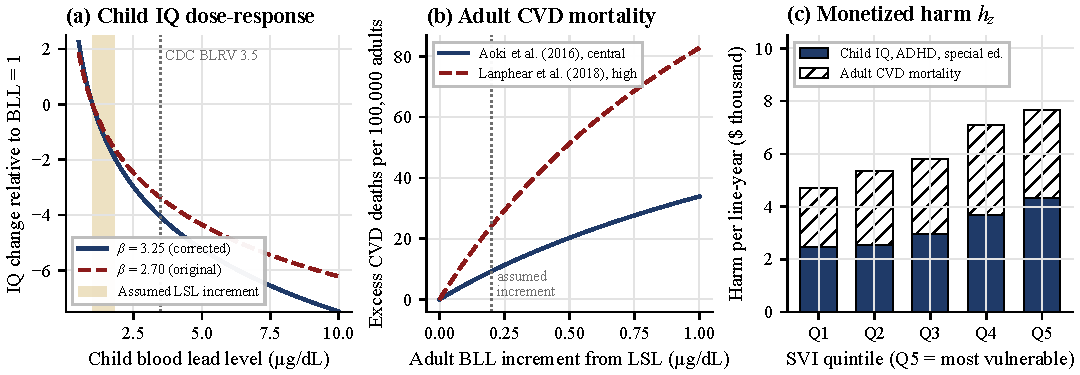
\includegraphics[width=\linewidth]{fig03_damage_functions.pdf}
\caption{Damage functions used to monetize exposure. (a) Log-linear child IQ dose--response with the corrected (3.25) and original (2.70) pooled coefficients; shading marks the assumed 0.8~\ugdl{} LSL increment. (b) EPA's health impact function for adult cardiovascular mortality under the Aoki (central) and Lanphear (high) coefficients. (c) Mean monetized harm per line-year by SVI quintile, computed from zone occupancy and expected lead share. Harm rises by about 60\% from the least to the most vulnerable quintile, driven mainly by child density.}\label{fig:damage}
\end{figure}

\subsection{Objective function}
\paragraph{Term A: health risk.} Present-value harm from lines still in service, counting a line
replaced in year $t$ as exposed for half of that year, is
\begin{equation}
H(\symbf x)=\sum_{t\in\Ts}\delta_t\sum_{z}h_zN_z\bigl(1-S_{z,t}-\tfrac12x_{z,t}\bigr)=H_0-A(\symbf x),
\label{eq:H}
\end{equation}
where $H_0$ is a constant and $A$ is avoided harm. The solver minimizes the constant-free form,
so the reported optimality gaps are measured on the decision-relevant part of the objective.

\paragraph{Term B: mobilization economies of scale.} Block programs incur a fixed setup cost $F$
(traffic control, permits, main-side excavation, crew relocation) and then a lower marginal cost:
\begin{equation}
C_t=\sum_{z}\bigl(F\,y_{z,t}+c^Bb_{z,t}+c^Oo_{z,t}\bigr),\qquad C=\sum_t\delta_tC_t .\label{eq:C}
\end{equation}
The average cost of a block batch of $n$ lines, $c^B+F/n$, is hyperbolic and declining
(\cref{fig:cost}), so cost is concave in volume; the fixed-charge formulation is its exact MILP
representation. With $c^B=\$31{,}000$ and $F=\$1.5$ million, a 500-line batch averages the reported
\$34,000, and block work beats one-off work ($c^O=\$39{,}000$) for batches above $n^*=F/(c^O-c^B)=188$.

\begin{figure}[t]\centering
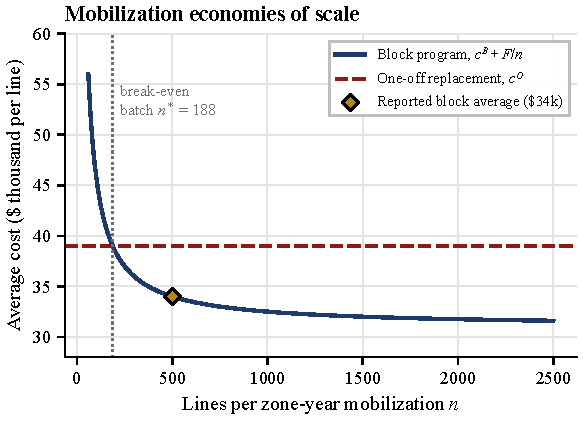
\includegraphics[width=0.6\linewidth]{fig04_cost_function.pdf}
\caption{Mobilization economies of scale implied by the fixed-charge cost model, $c^B+F/n$ with $c^B=\$31{,}000$ and $F=\$1.5$ million, compared with the reported \$39,000 one-off cost; the diamond marks the reported \$34,000 block average. Block delivery is cheaper than one-off work for any batch above 188 lines, so schedules that concentrate crews capture large savings.}\label{fig:cost}
\end{figure}

\paragraph{Term C: vulnerability-weighted equity penalty.}
\begin{equation}
E(\symbf x)=\sum_{z}\omega_z\,N_z\,\bigl(W_z-\bar W\bigr)^{+},\qquad \omega_z\in\bigl\{\SVI_z,\ \SVI_z^{\,3}/\overline{\SVI^3}\cdot\overline{\SVI}\bigr\},\label{eq:E}
\end{equation}
an $L^1$ analogue of a vulnerability-weighted upper semivariance of waits, linearized with
$d_z\geq W_z-\bar W$, $d_z\geq0$. The convex weight concentrates the penalty on the most vulnerable.

\paragraph{Combined objective.}
\begin{equation}
\min\quad \alpha_C\,C-\alpha_H\sum_{t,z}\delta_t\,\varphi_z\,h_zN_z\bigl(S_{z,t}+\tfrac12x_{z,t}\bigr)+\alpha_E\,\lambda\sum_z\omega_zN_zd_z ,\label{eq:obj}
\end{equation}
where $\varphi_z=1$ for utilitarian welfare and $\varphi_z=(\bar y/y_z)^{\eta}$ for Atkinson-type
distributional weights on median income $y_z$ with inequality aversion $\eta=1$, the approach of
HM Treasury's Green Book, which recommends an elasticity of 1.3 \citep{hmt2022}. All terms are present-value dollars.

\subsection{Constraints}
\begin{align}
&\textstyle\sum_tx_{z,t}=1 && \forall z && \text{(full replacement by }\bar T)\label{c:complete}\\
&N_zx_{z,t}=b_{z,t}+o_{z,t} && \forall z,t && \text{(volume split)}\label{c:split}\\
&m_zy_{z,t}\leq b_{z,t}\leq N_zy_{z,t} && \forall z,t && \text{(block linking)}\label{c:link}\\
&\textstyle\sum_zN_zx_{z,t}\leq K_t && \forall t && \text{(crew capacity)}\label{c:cap}\\
&\textstyle\sum_zy_{z,t}\leq Y && \forall t && \text{(concurrent block crews)}\label{c:crew}\\
&C_t\leq B_t && \forall t && \text{(capital budget)}\label{c:budget}\\
&\textstyle\sum_zN_z(S_{z,t}+x_{z,t})\geq\pi_tN && \forall t<\bar T && \text{(LCRI pace)}\label{c:pace}\\
&\tfrac{1}{N_{\EJ}}\textstyle\sum_{z\in\EJ}N_z(S_{z,t}+x_{z,t})\geq\tfrac1N\sum_zN_z(S_{z,t}+x_{z,t}) && \forall t && \text{(EJ floor)}\label{c:ej}\\
&d_z\geq W_z-\bar W,\quad d_z\geq0 && \forall z && \text{(excess wait)}\label{c:d}
\end{align}
Capacity follows the city's reported ramp (15,000, 19,000 and 22,000 lines in the first three years,
then 24,000, or 6,000 per quarter), $Y=34$, and the budget rises from \$450 million by \$40 million a
year to an \$820 million cap (\$\TotalBudget{} billion nominal over the horizon), a stylized blend of
DWSRF loans, revenue bonds and residual grants. The pace floor is $\pi_t=\max(0,t/\bar T-0.06)$.
Constraint \eqref{c:ej} guarantees that EJ zones are never behind the city as a whole.

\paragraph{Frontier.} To trace the welfare--equity frontier without choosing $\lambda$, we solve
\begin{equation}
\min\ C-A\quad\text{s.t.\ \eqref{c:complete}--\eqref{c:d}},\qquad
G(\symbf x)=\frac{1}{N_{\Qf}}\sum_{z\in\Qf}N_zW_z-\bar W\leq\varepsilon \label{eq:eps}
\end{equation}
over a grid of $\varepsilon$ \citep{haimes1971,mavrotas2009,ehrgott2005}. $G<0$ means the most
vulnerable quintile is served earlier than average. Reversing the inequality, with the EJ floor
relaxed, traces the branch on which vulnerable zones are pushed later.

\subsection{Structural results}
\begin{proposition}[Harm-ordered triage]\label{prop:smith}
With a uniform per-line cost and only constraints \eqref{c:complete} and \eqref{c:cap}, any schedule
that minimizes $H$ replaces zones in decreasing order of $h_z$.
\end{proposition}
\begin{proof}
Treat each line as a unit-length job with weight $h_z$. Exchanging one line of a lower-harm zone
scheduled earlier with one line of a higher-harm zone scheduled later changes $H$ by
$(h_{\text{low}}-h_{\text{high}})\sum_{s}\delta_s<0$ over the intervening years, while leaving cost
unchanged. This is the adjacent-interchange argument for weighted completion time
\citep{smith1956}.
\end{proof}

\begin{proposition}[Delay threshold]\label{prop:delay}
Deferring one line from year $t$ to $t+1$ changes the objective by
$\delta_t\bigl[h_z-c\,r/(1+r)\bigr]$. Early replacement is welfare-improving if and only if
$h_z>c\,r/(1+r)$.
\end{proposition}
\begin{proof}
Deferral adds one line-year of harm, $\delta_th_z$, and lowers the discounted cost from $\delta_tc$
to $\delta_{t+1}c=\delta_tc/(1+r)$, a saving of $\delta_tc\,r/(1+r)$.
\end{proof}
At $c=\$34{,}000$ the threshold is \$667 at 2\%, \$990 at 3\% and \$2,224 at 7\%. Zones holding
99.7\% of lines exceed the 3\% threshold and 99.4\% exceed the 7\% threshold, so absent budget and
crew limits the optimizer would replace nearly everything immediately. The schedule is therefore
shaped by scarcity, and the question is whom to serve first; the discount rate matters only for the
one or two least-harmed zones (\cref{sec:robust}).

\subsection{Solution procedure}
The model has 3,200 binaries, 9,760 continuous variables and about 10,000 constraints. It is solved
with CBC through PuLP \citep{mitchell2011pulp} (relative gap 0.1\%, absolute gap \$20 million,
200-second limit). Reported absolute gaps have a median of \$\MedGapMusd{} million and a maximum of
\$\MaxGapMusd{} million against objective values in the tens of billions (\cref{tab:scen}).
\Cref{alg:pipeline} summarizes the workflow.

\begin{algorithm}[t]
\caption{End-to-end pipeline}\label{alg:pipeline}
\KwIn{public raw files (\cref{tab:dict}); parameters (\texttt{config.py})}
\KwOut{schedules $\symbf x^\star$, frontier, sensitivity distributions, tables and figures}
Fetch raw data and verify checksums; join inventory to geocodes\;
Train tract-blocked classifier on verified lines; impute $P(\text{lead})$ for unknown lines\;
Build tract features (ACS, SVI, HOLC, CDPH); cluster action lines into zones $\Zs$\;
Compute $h_z$ by \cref{eq:harm}; define $\EJ$, $\Qf$\;
Simulate heuristics: empirical status quo, proportional pace, harm priority\;
\ForEach{scenario (CM, HW, EW, EW-convex, DW, robustness variants)}{solve \cref{eq:obj} s.t.\ \eqref{c:complete}--\eqref{c:d}\;}
$G^\star\leftarrow G(\symbf x^\star_{\mathrm{HW}})$; solve \cref{eq:eps} for $\varepsilon\in G^\star-\{1,\dots,6\}$ and the reversed problem for $\varepsilon\in\{G^\star+1.5,G^\star+3,0,2\}$\;
Evaluate all schedules on a common yardstick (central harm, $r=3\%$)\;
Draw \PsaN{} parameter vectors; re-evaluate fixed schedules; estimate consent models\;
\end{algorithm}

% =====================================================================
\section{Results}\label{sec:results}
% =====================================================================
% Results section; every number is a macro generated by src/analysis.py
\subsection{The status quo in the data}\label{sec:sq}
Before optimizing, we ask what the city has actually been doing. \Cref{fig:sq}a tabulates the
\NReplaced{} replacements completed in 2021--2025 and the \NRefused{} refusals of access by SVI
quintile. Two facts emerge. First, recent replacement activity has been mildly progressive: \ReplQE{}
replacements per 1,000 lines requiring action in the most vulnerable quintile against \ReplQA{} in the
least, consistent with the city's income-qualified Equity program and block work along main
replacements. The common presumption that request-driven programs are regressive does not describe
Chicago's recent record. Second, refusals rise steeply with vulnerability, from \RefQA{} to \RefQE{}
per 1,000 lines, tracking renter share (\RentQA\% to \RentQE\%). \Cref{sec:consent} shows that this
gradient survives controls. The equity problem in the data is therefore less about whom the city
chooses to serve than about whom it can reach.

\begin{figure}[t]\centering
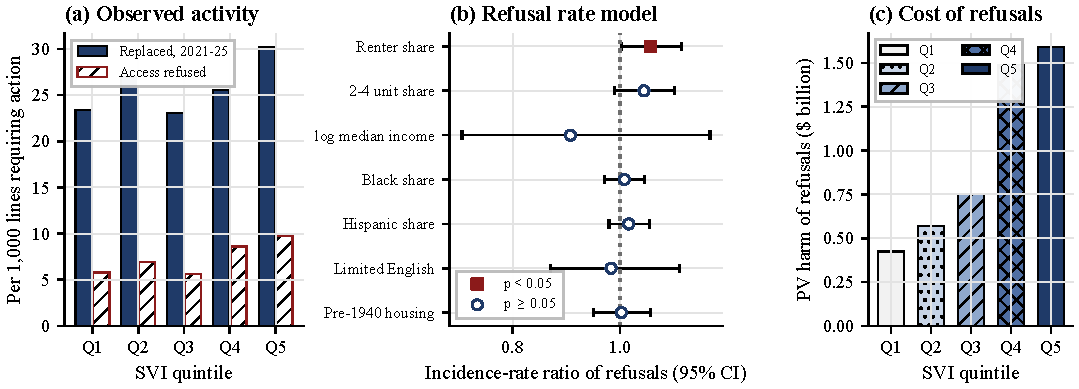
\includegraphics[width=\linewidth]{fig05_status_quo.pdf}
\caption{The status quo in the 2025 inventory. (a) Completed replacements (2021--2025) and refusals of access per 1,000 lines requiring action, by SVI quintile of the zone. (b) Incidence-rate ratios (95\% CI, standard errors clustered by community area) from a negative-binomial model of refusals per line across 608 tracts. (c) PV harm attributable to refusals under the health-welfare schedule, assuming refused lines wait until 2046. Recent replacements were mildly progressive, but refusals rise with vulnerability and renter share and concentrate the cost of refusals in the most vulnerable quintiles.}\label{fig:sq}
\end{figure}

\subsection{Scenario comparison}
We compare eight schedules (\cref{tab:scen}), all evaluated on a common yardstick (central harm,
$r=3\%$). Three are heuristics on the same budget and crew path: the \emph{status quo}, which allocates
capacity in proportion to each zone's empirical-Bayes smoothed 2021--2025 replacement rate;
\emph{proportional pace}, which advances every zone at the same rate; and \emph{harm priority}, which
fills capacity in descending $h_z$. All three use one-off delivery, because spreading crews across
the city never reaches block batch sizes; repricing the status quo with block pricing wherever a
zone-year reaches $m_z$ changes its cost by less than \$0.02 billion. Five are MILP solutions:
cost-minimizing (CM, $\alpha_H=0$), health-welfare (HW), equity-weighted with linear and convex SVI
weights (EW, EW-convex) and distributional weights (DW). All MILPs impose the EJ floor.

\begin{table}[t]\centering\scriptsize
\caption{Scenario outcomes ($r=3\%$; PV in \$ billion; waits are expected replacement years,
$t=1$ is 2027). $G$ is the Q5 wait gap (\cref{eq:eps}); $C$ is the concentration index of residual
child exposure ranked by SVI (negative = burden on the less vulnerable); $\mathcal G$ is the Gini of
exposure. Gap is the solver's absolute optimality gap (\$ million).}\label{tab:scen}
\setlength{\tabcolsep}{3pt}
\begin{tabular}{@{}lccccccccccc@{}}
\toprule
Schedule & PV $H$ & PV $C$ & PV $H{+}C$ & Done & $\bar W_{\EJ}$ & $\bar W_{\neg\EJ}$ & $G$ & $C$ & $\mathcal G$ & Block\,\% & Gap\\
\midrule
\csname @@input\endcsname tab_scenarios.tex 
\bottomrule
\end{tabular}
\end{table}

The status quo replaces \SQDonePct\% of the inventory by 2046 and finishes in \SQCompletion, missing
the deferred LCRI deadline. Its PV social cost is \$\SQSocial{} billion. The health-welfare schedule
finishes on time at \$\HWSocial{} billion, a saving of \$\DecTotal{} billion (\GainPct\%), of which
\$\DecHarmTotal{} billion is avoided harm and \$\DecCostTotal{} billion discounted capital. Nominal
capital spending falls from \$\SQNominal{} to \$\HWNominal{} billion. No one-off schedule can meet the
deadline at all: with block programs disabled the HW problem is infeasible, because 412,433 one-off
replacements at \$39,000 cost \$16.1 billion against \$\TotalBudget{} billion of capital over the
horizon.

One caveat on pricing deserves emphasis. The city's reported overall average (\$31,000) is below
both its block (\$34,000) and one-off (\$39,000) averages, which implies cheaper categories of work
within the current mix. If the status quo is priced at \$31,000 per line instead of the one-off rate,
its PV cost falls to \$\SQAltCost{} billion and its social cost to \$\SQAltSocial{} billion; the
health-welfare schedule still saves \$\SavingAlt{} billion (\SavingAltPct\%), now driven almost
entirely by avoided harm. The ordering result is robust to this choice; the size of the clustering
gain is not, and it should be re-estimated from CDWM contract data.

The saving decomposes cleanly. Moving from the status quo to harm priority with the same one-off
delivery saves \$\DecOrdering{} billion (\DecOrderPct\%): this is the value of ordering by risk.
Moving from harm priority to the HW solution saves a further \$\DecClustering{} billion
(\DecClusterPct\%): this is the value of clustering work into block programs and timing
mobilizations, which also lets the program finish on time. The cost-minimizing schedule captures
most of the clustering value but ignores harm and therefore leaves \$\CMHarm{} billion of PV harm
against \$\HWHarm{} billion under HW.

\subsection{Who is served first, and where}
\Cref{fig:sched} shows annual replacements by SVI quintile and \cref{fig:cmap} maps each zone's
expected replacement year. The status quo spreads capacity almost uniformly, so every zone waits
about the same (\SQWaitEJ{} years in EJ zones against \SQWaitNonEJ{} elsewhere). HW concentrates early
capacity on the West and Southwest Sides, where child density and confirmed lead are highest,
then moves outward; low-harm lakefront zones, dominated by large buildings with few small-diameter
lead services, come last. EJ zones are half complete by 2033, 84\% by 2039 and fully replaced by 2044 under HW
(\cref{fig:paths}), and
their expected replacement year is \HWWaitEJ{} against \HWWaitNonEJ{} for other zones.
Consistent with \cref{prop:smith}, the HW order tracks $h_z$, and because $h_z$ rises with SVI
(\cref{fig:damage}c), it is progressive without being told to be.

\begin{figure}[t]\centering
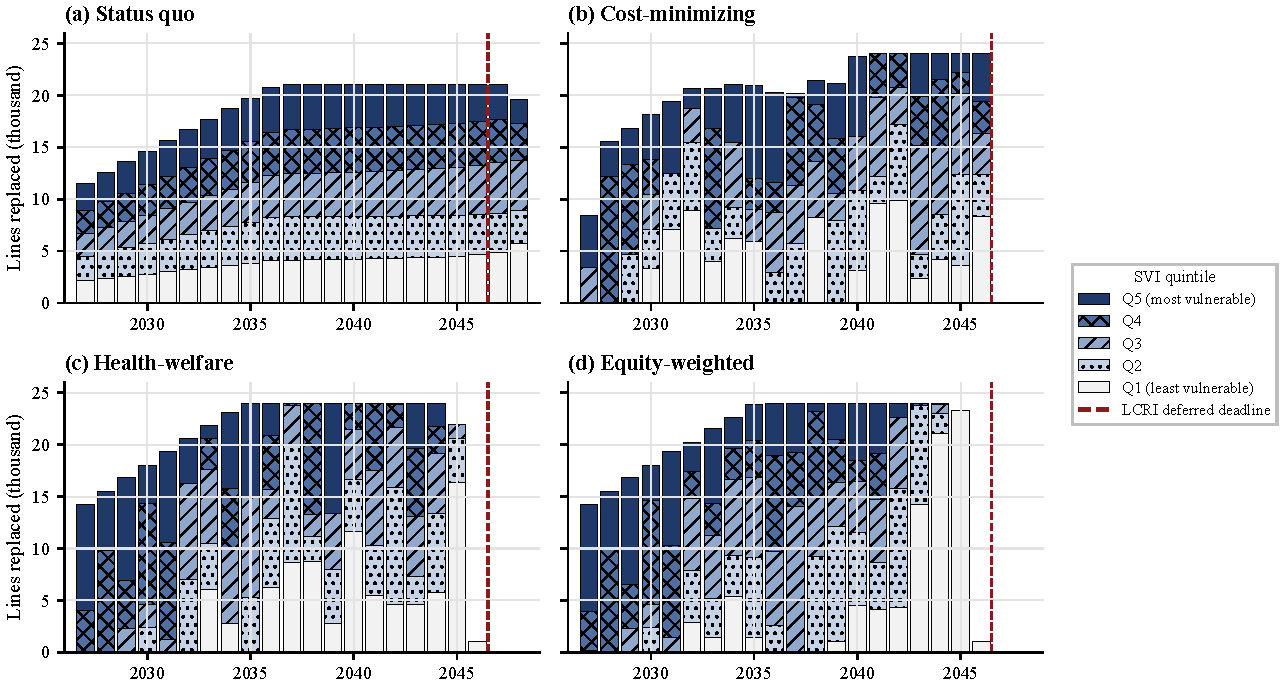
\includegraphics[width=\linewidth]{fig06_schedules.pdf}
\caption{Annual replacements by SVI quintile under four schedules: the empirical status quo (heuristic based on 2021--2025 replacement rates) and three MILP solutions (cost-minimizing, health-welfare and equity-weighted), all under the same budget and crew limits. The dashed line marks the end of the deferred LCRI schedule. The status quo spreads capacity evenly and misses the deadline, whereas the health-welfare schedule serves the most vulnerable quintile first and finishes on time.}\label{fig:sched}
\end{figure}

\begin{figure}[t]\centering
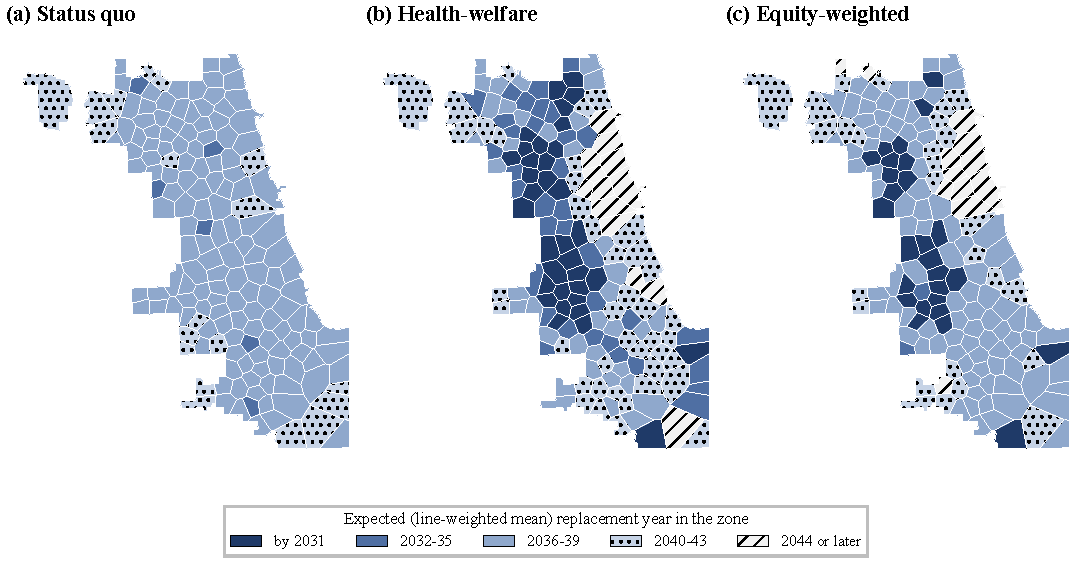
\includegraphics[width=\linewidth]{fig07_completion_maps.pdf}
\caption{Expected (line-weighted mean) replacement year of each of the 160 zones under the status quo, health-welfare and equity-weighted schedules; zones are Voronoi cells around the centroids of k-means clusters of lines requiring action. Optimized schedules replace the West and Southwest Sides first and the low-harm lakefront last, while the status quo leaves nearly every zone waiting until the late 2030s.}\label{fig:cmap}
\end{figure}

\begin{figure}[t]\centering
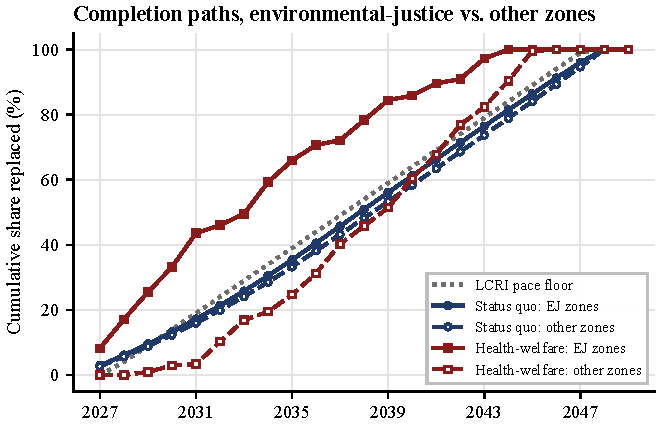
\includegraphics[width=0.7\linewidth]{fig08_completion_paths.pdf}
\caption{Cumulative share of lines replaced in environmental-justice zones (SVI at or above the 60th percentile) and other zones, status quo against the health-welfare schedule, with the LCRI pace floor. Under the health-welfare schedule EJ zones are half complete by 2033 and fully replaced by 2044, about four years before the status quo finishes them in 2048.}\label{fig:paths}
\end{figure}

\subsection{The welfare--equity frontier}
\Cref{fig:frontier} plots PV social cost against the Q5 gap. Three results stand out.

\emph{First, the welfare optimum is already progressive.} HW serves the most vulnerable quintile
\HWGapAbs{} years earlier than the citywide mean ($G=\HWGap$). Pricing harm correctly and serving the vulnerable first
are the same instruction over most of the range.

\emph{Second, delaying the vulnerable is dominated.} Every schedule to the right of HW, including the
reversed-constraint solutions with the EJ floor removed, has higher social cost and a worse gap. The
status quo and proportional pace sit far above and to the right of the frontier: no ethical weighting
that values both welfare and vertical equity would choose them over HW.

\emph{Third, along the frontier the trade-off is real but cheap.} Pushing $G$ from \HWGap{} to
\FrontMinGap{} years costs \$\FrontMinGapCost{} billion, under 2\% of social cost; beyond about $-8$
years the problem is infeasible under the capacity and pace constraints. Moving in the regressive
direction is also cheap (forcing $G=0$ costs \$\DomZeroCost{} billion), which is why equity cannot be
left to welfare arithmetic alone: the penalty for a regressive schedule is small enough that
administrative convenience could easily outweigh it. The EJ floor \eqref{c:ej} makes the
progressive ordering binding rather than merely optimal. The more consequential numbers lie off the
frontier: the \$\DecTotal{} billion between the status quo and HW, and the \$\RefCost{} billion cost of
refusals (\cref{sec:consent}).

\begin{figure}[t]\centering
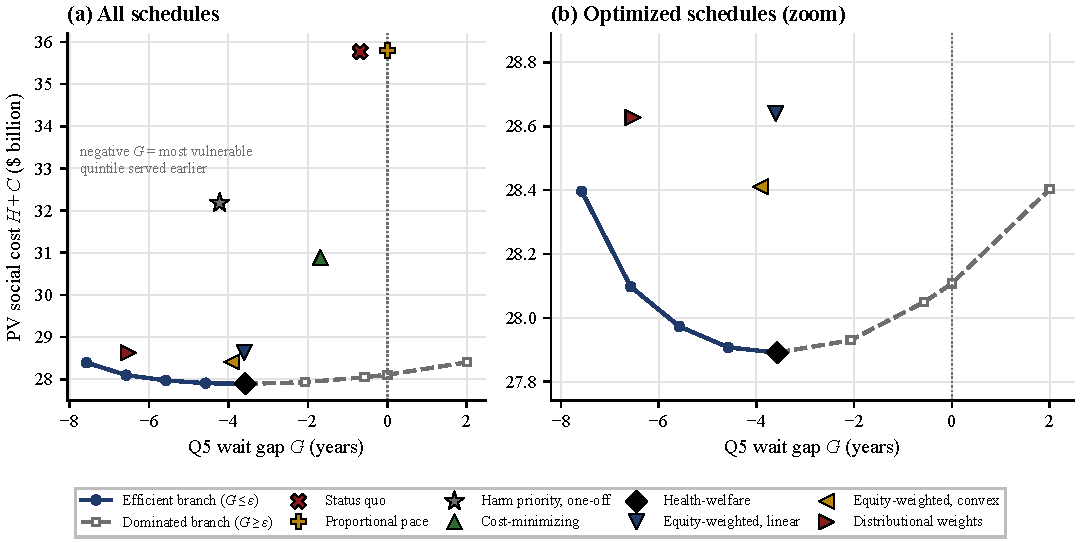
\includegraphics[width=\linewidth]{fig09_frontier.pdf}
\caption{Welfare--equity frontier traced with the $\varepsilon$-constraint method: each point on the efficient branch minimizes PV social cost subject to a bound on the Q5 wait gap $G$, and the dominated branch forces $G\geq\varepsilon$ with the EJ floor relaxed; markers show heuristic and MILP scenarios evaluated at central parameters and $r=3\%$. Panel (b) enlarges the optimized schedules. The welfare optimum is already progressive, schedules that delay the most vulnerable are dominated, and additional priority costs less than 2\% of social cost.}\label{fig:frontier}
\end{figure}

\subsection{Five equity frameworks}
The frameworks embed different normative commitments, and the data show how much those commitments
matter in practice. (i) \emph{Utilitarian} HW is progressive through the correlation of harm and
vulnerability. (ii) \emph{Distributional weights} with $\eta=1$ reweight harm toward low-income zones
and produce the most progressive schedule ($G=\DWGap$; EJ zones wait \DWWaitEJ{} years) at
\$\DWSocial{} billion on the utilitarian yardstick, \$0.74 billion above HW. (iii) The
\emph{linear SVI penalty} (EW) barely changes the Q5 gap ($G=\EWGap$) but lowers dispersion
(Atkinson $A_1$ from \HWAtkOne{} to \EWAtkOne): because \cref{eq:E} charges any zone that waits longer
than average and moderate-SVI zones carry substantial weight, it acts largely as a horizontal-equity
term that compresses waits. (iv) The \emph{convex SVI penalty} (EW-convex) concentrates weight on the
most vulnerable and moves $G$ to \ECGap{} at lower cost than EW. (v) The \emph{Rawlsian} limit, the
leftmost feasible frontier point, gives the most vulnerable quintile the maximum feasible priority
($G=\FrontMinGap$). The lesson for practice is that the functional form of an equity term is a
normative choice, not a technicality: a linear vulnerability-weighted penalty buys horizontal
equality, whereas distributional weights or convex weights buy priority for the worst off.

\subsection{The inequality-index paradox}\label{sec:paradox}
The symmetric inequality indices in \cref{tab:scen} rank the schedules almost exactly backwards.
Proportional pace has a Gini of zero and the status quo nearly so (\SQGini), while HW has the
highest Gini (\HWGini) and harm priority the highest Atkinson index (\POAtkOne). Gini and Atkinson
measure dispersion, and the status quo achieves low dispersion by delaying everyone, including the
most exposed, at a similar rate. Triage is unequal treatment of unequal risk, and a symmetric index
cannot tell progressive from regressive inequality.

Directional measures resolve the paradox. \Cref{fig:conc} plots concentration curves of residual
child exposure-years with children ordered from most to least vulnerable \citep{wagstaff1991}. The
status quo lies on the diagonal ($C=\SQConc$); HW lies well below it ($C=\HWConc$), so the most
vulnerable children bear much less than their population share of remaining exposure. An
algorithmic-equity audit that relies on Gini or Atkinson indices alone would penalize exactly the
triage that environmental justice calls for. Audits should report a directional statistic: the gap
$G$, a concentration index, or completion paths by vulnerability.

\begin{figure}[t]\centering
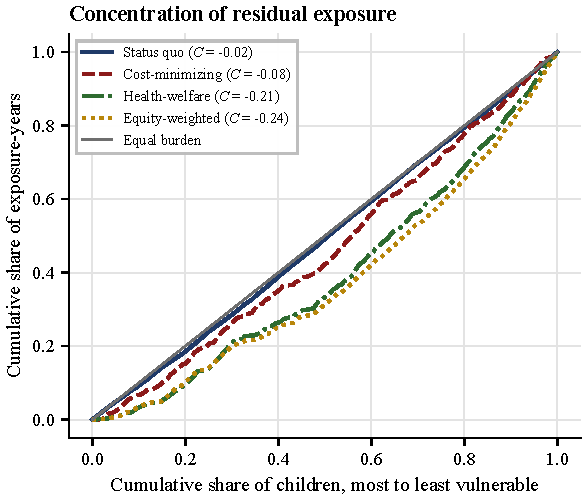
\includegraphics[width=0.6\linewidth]{fig10_concentration.pdf}
\caption{Concentration curves of residual child exposure-years, computed from each schedule's yearly replacement shares and zone child density, with children ordered from most to least vulnerable; $C$ is the concentration index. The status quo spreads remaining exposure almost evenly ($C\approx0$), whereas optimized schedules place it on the less vulnerable, which symmetric Gini and Atkinson indices fail to distinguish.}\label{fig:conc}
\end{figure}

\subsection{Robustness of the schedule}\label{sec:robust}
\Cref{tab:robust} re-solves HW under alternative discount rates, benefit tiers and a tap-lead
gradient taken from \citet{huynh2024}. The schedule itself is remarkably stable. Evaluated on the
common yardstick, every variant is within \$0.3 billion of HW, and the Q5 gap ranges only from
\HChGap{} to \HHuGap{} years. The discount rate barely moves the order because zones holding more than 99\% of lines
have harm above the \cref{prop:delay} threshold even at 7\%, so budgets rather than discounting
determine timing. The tap-lead gradient, which raises harm in heavily Hispanic zones on the Southwest Side,
moves some of those zones earlier and narrows the gap, a reminder that better exposure data could
reorder the middle of the schedule. What is uncertain is the size of the benefits, not the sequence.

\begin{table}[t]\centering\small
\caption{Robustness of the health-welfare schedule. ``Own'' is PV social cost under the variant's own
assumptions; ``Common'' evaluates the variant's schedule under the central assumptions at 3\%.}
\label{tab:robust}
\begin{tabular}{@{}lcccccc@{}}
\toprule
Variant & Own $H{+}C$ & Common $H{+}C$ & $G$ & $\bar W_{\EJ}$ & $\bar W_{\neg\EJ}$ & Block\,\%\\
\midrule
\csname @@input\endcsname tab_robust.tex 
\bottomrule
\end{tabular}
\end{table}


% =====================================================================
\section{Economic analysis}\label{sec:econ}
% =====================================================================
\subsection{Per-line net present value}
For a line with harm $h$, lifecycle $L=30$ years and social discount rate $r$,
\begin{equation}
\mathrm{NPV}(r,c)=h\,\mathcal A(r,L)-c,\qquad \mathcal A(r,L)=\frac{1-(1+r)^{-L}}{r},\qquad
\mathrm{BCR}=\frac{h\,\mathcal A(r,L)}{c}.\label{eq:npv}
\end{equation}
OMB Circular A-4 prescribed 3\% and 7\% rates in 2003 and a 2\% rate in its 2023 revision
\citep{omb2003a4,omb2023a4}; which guidance governs federal analysis has shifted across
administrations, so we report all three. \Cref{tab:npv} reports the citywide BCR by benefit tier.

\begin{table}[t]\centering\small
\caption{Citywide per-line benefit--cost ratio by benefit tier, unit cost and discount rate
($L=30$ years).}\label{tab:npv}
\begin{tabular}{@{}llccc@{}}
\toprule
Benefit tier & Cost per line & $r=2\%$ & $r=3\%$ & $r=7\%$\\
\midrule
\csname @@input\endcsname tab_npv.tex 
\bottomrule
\end{tabular}
\end{table}

Replacement passes the benefit--cost test in every cell. Under the most conservative
combination (child benefits only, \$39,000 one-off cost, 7\%) the BCR is \BCRChildThirtyNineSeven;
in the central case at Chicago's \$31,000 average it is \BCRCentralThirtyOneThree{} at 3\%. Chicago's
cost premium therefore does not threaten the case for replacement, but it does cost real money: at
the national \$10,000 benchmark the central BCR would be \BCRCentralTenThree. Because benefits are
large relative to costs everywhere, the efficiency question is not whether to replace but how to
sequence and how to contain cost, which is where the optimization earns its value.

\paragraph{Municipal borrowing.} The PV at social rate $r$ of a level-payment loan of principal $c$
at rate $i_b$ over $n$ years is
\begin{equation}
\mathrm{PV}_{\mathrm{fin}}(c;i_b,r,n)=c\,\frac{i_b}{1-(1+i_b)^{-n}}\,\mathcal A(r,n).\label{eq:fin}
\end{equation}
\begin{table}[h]\centering\small
\caption{PV of financing a \$31,000 line over 30 years.}\label{tab:fin}
\begin{tabular}{@{}lccc@{}}
\toprule
Social rate & Cash & DWSRF loan (1.5\%) & Revenue bond (5.0\%)\\
\midrule
\csname @@input\endcsname tab_finance.tex 
\bottomrule
\end{tabular}
\end{table}
At a 3\% social rate a subsidized DWSRF loan lowers the effective cost of a line by about 18\%, while
a 5\% revenue bond raises it by about 28\% (\cref{tab:fin}). Slow drawdown of subsidized federal
credit \citep{wttw2025} is therefore not a neutral delay: it forfeits the cheapest capital available.

\subsection{Probabilistic sensitivity analysis}\label{sec:psa}
We draw \PsaN{} parameter vectors: IQ slope uniform on [2.70, 3.25]; value per IQ point uniform
on EPA's [\$38,404, \$46,204]; child and adult BLL increments triangular on [0.4, 0.8, 1.5] and
[0.1, 0.2, 0.4]~\ugdl; the CVD function drawn with equal probability from the Aoki or Lanphear
confidence ranges; VSL $\pm25\%$; $c^B\in[\$27\mathrm k,\$35\mathrm k]$, $c^O\in[\$35\mathrm k,\$45\mathrm k]$,
$F\in[\$0.75\mathrm M,\$3\mathrm M]$; and $r\in\{2,3,7\}\%$. Each fixed schedule is re-evaluated
under every draw. The health-welfare schedule has lower social cost than the status quo in
\PsaHWbeatsSQ\% of draws, with a median saving of \$\PsaSaveMed{} billion (90\% interval
\$\PsaSaveLo{} to \$\PsaSaveHi{} billion), and is the best of the six evaluated schedules in
\PsaHWbest\% of draws. The citywide BCR at \$31,000 has a median of \PsaBcrMed{} (90\% interval
\PsaBcrLo{} to \PsaBcrHi) and falls below one in \PsaBcrBelowOne\% of draws (\cref{fig:psa}). The
one-way analysis (\cref{fig:npv}b) shows that the CVD dose--response choice dominates the
uncertainty, followed by the exposure increments and the discount rate; the IQ slope and its
valuation matter least.

\begin{figure}[t]\centering
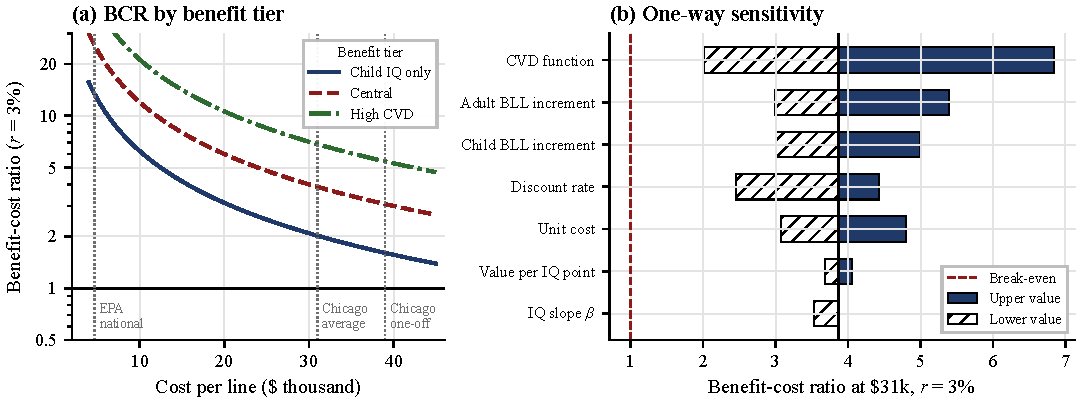
\includegraphics[width=\linewidth]{fig11_npv.pdf}
\caption{(a) Citywide per-line benefit--cost ratio against unit cost for three benefit tiers at $r=3\%$, computed from line-weighted mean harm over a 30-year life. (b) One-way sensitivity of the BCR at \$31,000 and 3\% to each uncertain input across its stated range. Replacement passes the benefit--cost test at Chicago's costs in every tier, and the cardiovascular dose--response choice is the largest source of uncertainty.}\label{fig:npv}
\end{figure}

\begin{figure}[t]\centering
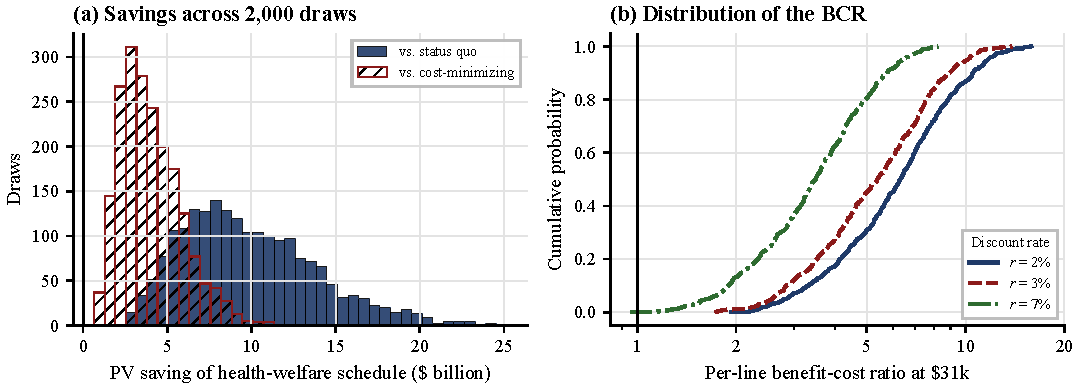
\includegraphics[width=\linewidth]{fig12_psa.pdf}
\caption{Probabilistic sensitivity analysis from 2,000 Monte Carlo draws of dose--response, valuation, cost and discount-rate parameters, with each fixed schedule re-evaluated in every draw. (a) PV saving of the health-welfare schedule relative to the status quo and to the cost-minimizing schedule. (b) Cumulative distribution of the citywide BCR at \$31,000 by discount rate. The health-welfare schedule beats the status quo in every draw (median saving \$9.3 billion), and the BCR falls below one in only 0.1\% of draws.}\label{fig:psa}
\end{figure}

\subsection{Split ownership, consent and the tenant externality}\label{sec:consent}
A replacement requires the property owner's consent for work on private property. In a rental
building, the person who consents is not the person who drinks the water. Let an owner face private
cost share $s$ of $c$, a hassle cost $\kappa$ and household benefit $B$. The owner consents iff
\begin{equation}
\theta B-sc-\kappa\geq0,\qquad
\Pr(\text{consent})=\Lambda\Bigl(\frac{\theta B-sc-\bar\kappa}{\sigma}\Bigr),\label{eq:consent}
\end{equation}
with $\kappa\sim\mathrm{Logistic}(\bar\kappa,\sigma)$. Owner-occupants internalize the benefit
($\theta=1$); a landlord captures only the share $\theta<1$ that is capitalized into rents or
values. The wedge $(1-\theta)B$ is a positive externality, and the public share needed to align
private and social incentives is $1-s^\star=1-(\theta B-\kappa)/c$, which rises toward one as
$\theta\to0$. Chicago's Equity, Daycare, Block and Leak programs replace lines at no cost to the
owner, and only the Homeowner-Initiated program is owner-paid, with permit fees of up to \$5,000
waived \citep{cdwm2024ccr}. The free Equity program, however, is limited to owners of houses and
two-flats with incomes below 80\% of area median income, so a landlord of a larger rental building
generally obtains a free replacement only when the city happens to schedule block work on the
street. For rental property, the program design keeps $s$ high outside block work, and the remaining
levers in \cref{eq:consent} are $\theta$ (lead disclosure at lease and sale capitalizes the hazard)
and $\kappa$ (streamlined consent or a statutory right of entry).

\paragraph{Evidence.} The inventory records \NRefused{} refusals of access. Across \ConsN{} tracts
with at least five attempts (\ConsAttempts{} attempts, \ConsRefusals{} refusals), we estimate a
binomial model of the refusal share among attempts and a negative-binomial model of refusals per
line requiring action, both with standard errors clustered by community area:
\begin{equation}
\log\mathbb E[\text{Refusals}_j]=\log N_j+\symbf X_j'\symbf\gamma,\qquad
\mathrm{logit}\,\Pr(\text{refuse}\mid\text{attempt})_j=\symbf X_j'\symbf\beta .\label{eq:econ}
\end{equation}
Renter share is the only covariate significant at 5\% in the rate model: each 10-point increase
raises the refusal rate by a factor of \ConsIRR{} (95\% CI \ConsIRRlo{} to \ConsIRRhi, $p=\ConsIRRp$),
conditional on income, race and ethnicity, limited English, housing age and two-to-four-unit
structure share (\cref{tab:consent}). In the share model the coefficients have the expected signs
but are imprecise. The bivariate share model implies refusal probabilities of \PRefOwner\% in an
all-owner tract and \PRefRenter\% in an all-renter tract. The pattern is consistent with the
principal--agent mechanism, although tract-level data cannot separate landlord refusal from other
correlates of renting.

\begin{table}[t]\centering\small
\caption{Determinants of refusals of access, tract level. Standard errors clustered by community
area in parentheses. $^{\dagger}p<0.10$, $^{*}p<0.05$, $^{**}p<0.01$.}\label{tab:consent}
\begin{tabular}{@{}lcccc@{}}
\toprule
 & \multicolumn{2}{c}{Binomial: share of attempts} & \multicolumn{2}{c}{Neg.\ binomial: rate per line}\\
\cmidrule(lr){2-3}\cmidrule(lr){4-5}
Covariate & Coef. & (SE) & Coef. & (SE)\\
\midrule
\csname @@input\endcsname tab_consent.tex 
\bottomrule
\end{tabular}
\end{table}

\paragraph{Welfare cost of refusals.} Using empirical-Bayes refusal shares by zone (citywide
\RefRho\%; \RefRhoQO\% in the least and \RefRhoQF\% in the most vulnerable quintile) and assuming
refused lines wait until the end of the horizon, refusals add \$\RefCost{} billion of PV harm to the
health-welfare schedule, \RefCostEJ\% of it in EJ zones (\cref{fig:sq}c). That is about ten times
the welfare cost of the most demanding feasible equity constraint (\$\FrontMinGapCost{} billion) and
\RefCostShareGain\% of the entire gain from optimization, which is why consent policy, not the
sequencing rule, is the binding equity margin.

% =====================================================================
\section{Policy implementation, cultural receptivity and governance}\label{sec:policy}
% =====================================================================
\subsection{Institutional bottlenecks}
Three frictions determine whether an optimal schedule can be executed. \emph{Procurement.} Chicago's
unit cost is two to six times that of peer cities \citep{icn2026cost}. Our model shows why the
structure of contracts matters as much as their level: the gain from clustering depends on
$c^O-c^B$ and $F$, and a schedule that spreads crews thinly across the city, as both the status quo
and proportional pace do, never reaches the batch sizes at which block pricing applies (the status
quo uses block pricing for \SQBlock\% of lines). Multi-year, zone-bundled contracts with published
unit prices are the procurement analogue of \cref{eq:C}. \emph{Permitting.} Each line crosses public
right-of-way and private property; zone-level master permits convert thousands of approvals into one
per mobilization. \emph{Right of entry.} Refusals are concentrated where renters are concentrated;
in \cref{eq:consent} the hassle term $\kappa$ is the parameter administrative design can move fastest.

\subsection{Community trust and cultural buy-in}
Algorithmic scheduling can reproduce injustice if residents experience it as opaque, and the
communities the model prioritizes have the strongest historical reasons for mistrust of government
water and health systems. Three practices address this. First, the prioritization rule, its inputs
and the annual schedule should be public, so residents can verify that a zone is first because of
measured risk rather than political favor. Second, outreach should match the population served:
multilingual notices (the city's notification of about 900,000 owners and occupants was only 7\%
complete by July 2025; \citealp{wttw2025}), trusted messengers through schools, clinics and
congregations, and door-to-door consent drives timed to the crew's arrival. Because Black and
Hispanic blocks are under-tested \citep{huynh2024}, scheduling from voluntary test requests would
reproduce bias; scheduling from the inventory, as here, avoids it. Third, the jobs should stay in the
neighborhoods: HUD's Section 3 rule sets benchmarks of 25\% of labor hours by Section 3 workers and
5\% by targeted workers \citep{hud2020section3}, which can be applied to LSLR contracts so that a
twenty-year capital program is also a workforce pipeline.

\subsection{Policy recommendations}
\begin{enumerate}[leftmargin=1.4em]
\item \textbf{Mandatory Full Replacement and Right-of-Entry Ordinance.} Require replacement of both
sides of every LSL in a scheduled zone mobilization; deem consent given after two documented
notices to owner and occupants in their language; authorize CDWM entry for private-side work. This
targets the \$\RefCost{} billion refusal cost and the renter gradient in \cref{tab:consent}.
\item \textbf{Zero-Cost Replacement and Water Affordability Rider.} Codify no-cost replacement for
owner-occupied and rental properties alike; finance through DWSRF credit first and revenue bonds
second (\cref{tab:fin}); cap the LSLR-attributable water and sewer rate increase for households
below 200\% of the federal poverty line through an income-based discount, so the program is not
financed regressively through volumetric rates; and require lead disclosure at lease signing and sale.
\item \textbf{Algorithmic Transparency and Equity Audit Ordinance.} Require CDWM to schedule with a
published, risk-based model; enforce the non-discrimination floor \eqref{c:ej}; and publish each
year the Q5 wait gap $G$, EJ and non-EJ completion paths and the concentration index of residual
exposure. Because symmetric indices misread triage (\cref{sec:paradox}), the ordinance should
specify directional metrics.
\item \textbf{Unit-Cost Benchmarking and Local Hiring Ordinance.} Require zone-bundled, multi-year
contracts with public unit prices benchmarked annually against peer utilities, with a target path
toward the peer median, and apply Section 3 labor-hour benchmarks with apprenticeship slots for
residents of priority zones.
\end{enumerate}

% =====================================================================
\section{Limitations and conclusion}\label{sec:conc}
% =====================================================================
The analysis has five main limitations. (i) Tap sampling is not public at address level, so
exposure per lead line is uniform in the central case. (ii) Dose increments from LSL water to blood
lead are assumptions, varied widely in the PSA. (iii) Zones are geometric clusters of lines rather
than hydraulic segments of the main network; parcel-level scheduling with main adjacency would
sharpen the clustering estimates. (iv) The refusal models are tract-level associations, and the
refusal cost assumes refused lines wait until 2046. (v) Costs, mobilization and budgets are
calibrated to reported averages rather than contract data. Each is addressable with the pipeline
provided.

The qualitative conclusions follow from structure that the data confirm rather than from any single
parameter. Benefits exceed costs by a wide margin, so scarcity, not efficiency, shapes the schedule.
Harm, child density and vulnerability are positively correlated, so pricing harm correctly serves
the vulnerable first, and delaying them is dominated. Spreading crews thinly forfeits the economies
of scale that a fixed-charge cost structure rewards, so the status quo is both slower and more
expensive. And refusals concentrated among renters are a larger equity problem than any remaining
sequencing choice. The policy debate should shift from whether to prioritize vulnerable
neighborhoods to how quickly the city can contain unit costs and secure consent so that the
prioritized schedule is actually delivered.

\section*{Data and code availability}
All code is in \texttt{src/}. \texttt{bash setup.sh} builds the environment (Appendix~\ref{app:setup});
\texttt{python src/fetch\_data.py} downloads the raw data; \texttt{python src/run\_all.py} runs the
ETL, solves the scenarios, and regenerates every figure, table and in-text number; and
\texttt{latexmk -xelatex paper/main.tex} rebuilds the typeset manuscript and \texttt{python paper/build\_docx.py} the Word version.

\section*{Acknowledgments}
The address-level inventory and geocoding were made public by Inside Climate News, Grist and WBEZ.
HOLC data are from Mapping Inequality (CC BY-NC).

\bibliographystyle{plainnat}
\bibliography{../bib/references}

\appendix
\section{Local environment setup (Section 0)}\label{app:setup}
\lstinputlisting[language=bash]{../setup.sh}

\section{ETL pipeline}\label{app:etl}
\lstinputlisting[language=Python]{../src/etl_pipeline.py}

\section{Optimization model}\label{app:opt}
\lstinputlisting[language=Python,firstline=89,lastline=158]{../src/optimize.py}

\section{Target journal and typesetting specification}\label{app:journal}
\begin{itemize}[nosep]
\item \textbf{Target:} \emph{Environmental Science \& Policy} (Elsevier); alternate \emph{Nature Water}.
Research article with structured abstract, 6--8 keywords, highlights (3--5 bullets of at most 85
characters) and a graphical abstract (\cref{fig:frontier}).
\item \textbf{Class:} Elsevier \texttt{elsarticle} with \texttt{[preprint,12pt,authoryear]} for
review; this preprint uses \texttt{article} with identical content.
\item \textbf{Citations:} BibTeX, author--year; \verb|\citet| in text and \verb|\citep|
parenthetically; DOIs for all journal articles, each verified against Crossref.
\item \textbf{Typography and mathematics:} Times New Roman for text, figures and mathematical
letters (\texttt{fontspec}, \texttt{unicode-math}); every displayed equation numbered; sets
calligraphic, vectors bold, units through \texttt{siunitx}; vector PDF figures.
\end{itemize}

\section{BibTeX database}\label{app:bib}
\lstinputlisting[numbers=none]{../bib/references.bib}

\end{document}
